%!TEX root = ../thesis.tex

\chapter{Case study design} \label{chap:researchdesign}

In the previous chapter, I reviewed relevant theory and methods for functional analysis of language use in \glspl{OSG}, centring on \gls{CL} as a potential approach and \gls{SFL} as a theory of language. This chapter introduces the case study of the thesis---a \gls{corpus}\hyp{}based analysis of an online \gls{bipolar} \glslink{OSG}{support group}. In the sections that follow, I describe the site selection and ethical considerations, data collection, and \gls{corpus} building processes. I then describe the analytical methods used in the investigation, and the development of \texttt{corpkit}, a \texttt{Python} module for building and interrogating \glspl{corpus}, and for editing and visualising interrogation results. Its core functionality and user interfaces are summarised. Justifications are provided for key choices throughout the chapter.

%There are currently dozens of bipolar disorder forums online. To locate the most suitable for analysis, I followed the method of \textcite{sillence_communicating_2012}. After locating eleven open-access bipolar disorder forums through search engine queries and exploring the basic infrastructure and content of each, \emph{Healthboards} was selected as the most suitable site for analysis. This choice was made for a number of reasons. First is its popularity: the \gls{Forum} is large and relatively active, having received over 66,000 \glspl{post} from thousands of unique users at the time of data collection. The presence of a number of users with thousands of \glspl{post} was also a prerequisite filled by the \gls{Forum}, as `veteran' members were required for the planned Investigation C. Second, the site has a global (English-speaking) focus: the presence of sizeable groups of users from most Anglophone countries was perceived to be a benefit. That said, the main nationality of Healthboards users is U.S. American, in part due to the site's use of U.S. American medication names, but also likely due to the existence of other bipolar disorder websites specifically designed for the UK (e.g. \emph{BipolarUK}), Australia (\emph{Beyond Blue, Blueboards}), etc.

%A third benefit of Healthboards is that the bipolar disorder forum is just one of many similarly structured boards for other health concerns. This allows potential future investigations to compare sub-forums, or analyse a group of sub-forums (e.g. all mental health forums) simultaneously. Fourth, Healthboards does not automatically delete old \glspl{post}, and has not undergone any renovations that have forced members to create new accounts. Thus, I had access to \glspl{post} dating back to the beginning of the message board, and could track individual users more accurately \cite{danescu-niculescu-mizil_no_2013}. Finally, at the time of data collection, Healthboards had no identifiable policy prohibiting web-crawling or re-use of content.

%\cite{danescu-niculescu-mizil_no_2013 In particular, it would be interesting to investigate how the patterns of linguistic change are affected by engagement in multiple communities, as well as how users that are members of multiple communities transfer norms and conventions between communities.

\section{Site description and selection}

The case study of this thesis is a \gls{corpus} comprised of 13 years of \glspl{post} to a once\hyp{}popular \gls{OSG} for those living with \gls{bipolar}---a mental disorder characterised by oscillation between elevated and depressed moods \cite{anderson_bipolar_2012}. The \gls{forum} has been online since 2001, with very little change to the interface or account system. As such, the \gls{Mode} dimension of the \gls{Forum} has stayed largely static, and many \glslink{member}{users} have participated using the same account details for a number of years. The \gls{Forum} is a part of a larger architecture of health-related \glslink{forum}{boards}, many of which were created at different points in time. \glslink{member}{Users'} accounts work site\hyp{}wide; as such, many of the contributors to the \glslink{forum}{Bipolar Forum} have also created \glspl{post} elsewhere. At the time of data collection (early 2014), the \glslink{forum}{Bipolar Forum} had over 5700 users, with a handful of `veteran' \glslink{member}{users} recording over a thousand \glspl{post} (see Figure \ref{fig:counts}). By the time the \gls{Forum} content was harvested, it was in a state of decline: 2013 saw a total of only 119 new \glspl{thread}, compared with over 1,699 during its peak in 2007 (see Figure \ref{fig:stage_year}). The average number of replies to \glspl{thread} has also dropped dramatically since its peak (from 7.59 in 2009 to 1.40 in 2013---see Figure \ref{fig:avg_replies}). Observation of the \gls{Forum} between 2014--2016 suggests that these trends have continued.\endnote{Similar patterns of declining forum use have been noted elsewhere in online community literature: in a study of a forum dedicated to the band \emph{Belle and Sebastian} \cite{deller_decade_2014}, interviewed \gls{Forum} users suggest that both social (changing interests, lack of time) and technological (obsolescence of forums) factors contribute to a rapid decline in use.}

% make gls work in section title
\subsubsection{Forum architecture}

The \glslink{Forum}{community} is a prototypical example of a \emph{vBulletin}-powered message board, with a main page showing the most recent active \glspl{thread}, and with each \gls{thread} containing a set of chronologically ordered \glspl{post}. \glslink{member}{Users} are able to send private messages, search \gls{Forum} contents, and show \glspl{post} related to specific medications or symptoms. The \glslink{Forum}{community} has explicit rules (in the form of \emph{sticky \glspl{post}} at the top of the message board) stating that new \glslink{member}{users} should not provide offline contact information, or request diagnoses from other \glspl{member}. \Glspl{post} breaking rules could be edited or deleted by moderators, who can also comment on their moderation decisions. If provided, a \glslink{member}{user}'s gender and\slash or location are displayed beside his\slash her \gls{post}, alongside the username and current postcount.

\subsubsection{Forum users}

%todo: copy edit
Based on location metadata, \glspl{member} are overwhelmingly from Anglophone countries (see Figure \ref{fig:map}). Most members believe themselves to have \gls{bipolar}, or have at some stage been diagnosed with \glslink{bipolar}{bipolar}. Less common are family, friends and partners of somebody believed to have the condition. This distribution is similar to the \gls{forum} investigated by \textcite{vayreda_social_2009}. Notably, there is a related \gls{forum} for `Family \& Friends of Mentally Ill' whose use is encouraged in an administrator's sticky \gls{post}. Health professionals are either not present in the community or do not identify themselves as such. The \gls{Forum}'s rules explain that the site is for \glspl{consumer}, rather than professionals:

\begin{quote} \singlespacing \small
Do not register or post your past, current or future health topic profession in any manner. The boards are to be used for PATIENT opinions, only. Professional titles lend undue weight to what is to be only your opinion. Health profession titles are not allowed. % http://www.healthboards.com/boards/faq.php?faq=faq_hb#faq_new_faq_item
\end{quote}
%
Concordancing the terms used by \gls{Forum} \glspl{member} for health professionals (\emph{doctor}, \emph{doc}, \emph{pdoc}, \emph{tdoc}, \emph{gp}, \emph{shrink}, \emph{psychologist}, etc.) revealed no instances of \glslink{member}{users} claiming to have formal medical training.

%todo: make sure these look nice, hopefully at top and bottom of page
\begin{figure}[t]
\centering
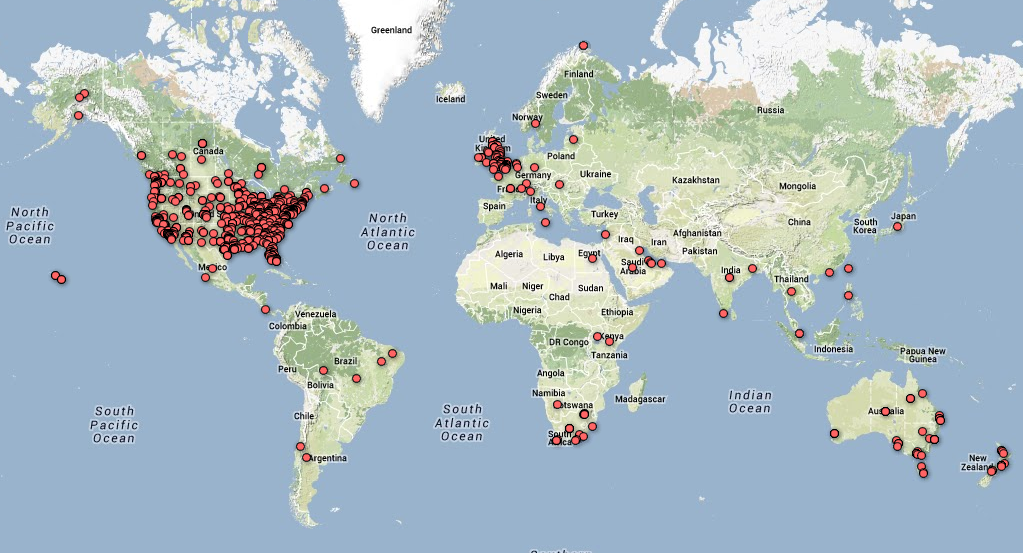
\includegraphics[width=0.61\linewidth]{../images/map3}
\caption{Stated locations of members}\label{fig:map}
\end{figure}

\begin{figure}[b]
\centering
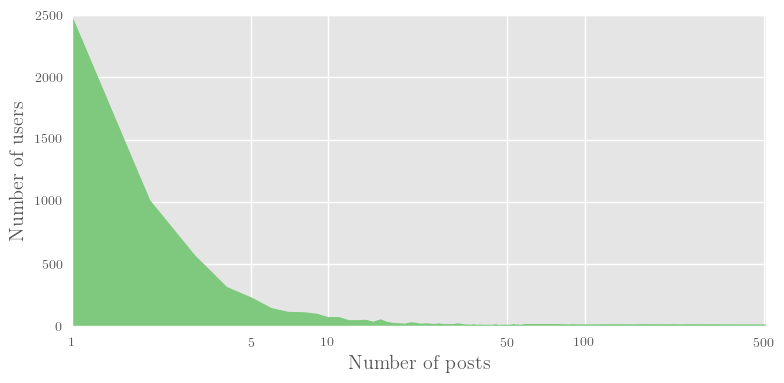
\includegraphics[width=0.70\linewidth]{../images/best-posts-users}
\caption{Total members by postcount}\label{fig:counts}
\end{figure}

Unlike in Maclean et al's analysis of \emph{Forum77} \parencite*{maclean_forum77:_2015}, \glslink{member}{users} who were active at the time of data collection were not excluded from the dataset. A potential effect of this is that the ratio of veteran to non\hyp{}veteran \glslink{member}{users} is slightly skewed toward non\hyp{}veteran \glslink{member}{users}, as some currently active members may eventually progress to become veteran members in the future.
%todo: removed because point already made?
%That said, the \glslink{forum}{Bipolar Forum} was in a state of rapid decline at the time of data collection. Therefore, very few \glspl{member} would have ultimately been removed according to the criteria of recent activity.

One final consideration regarding the \glslink{member}{user} base is that nothing prevents \glslink{member}{users} from creating and \glslink{post}{posting} from multiple accounts. As such, following \textcite{de_choudhury_discovering_2016}, the terms \emph{\glslink{member}{user}}, \emph{\gls{member}} and \emph{\glslink{member}{contributor}} refer more specifically to \glslink{member}{users'} accounts than to actual people who use the \glslink{Forum}{board}. That said, there is no evidence to suggest, and no reason to believe, that \glslink{member}{users} create and \gls{post} under multiple accounts.

\subsection{Justification for site selection}

The \gls{Forum} is a typical example of a large online \glslink{forum}{message board}. As discussed in Chapter \ref{chap:onlinehealth}, these kinds of communities are well\hyp{}studied, allowing more reliable connection of findings to earlier research into \glspl{OSG} than would be the case if the selected site was from an emerging \gls{mode} of \gls{CMC}. The fact that the \gls{Forum} has undergone few structural changes since 2001 is particularly useful, as it eliminates a potential confounding variable, where longitudinal changes in language use may be affected by changes in the ways \glslink{member}{users} create and transmit messages. While it is possible that hardware changes (faster web access, increased mobile usage, etc.) could have effects on language use, such effects also occur in other non\hyp{}researcher\hyp{}constructed communities. Compared to social networking sites and mobile apps, both of which typically undergo constant interface redesign, the \glslink{Forum}{Bipolar Forum} can be seen as relatively stable over time.

An important reason for selecting the \gls{Forum} is its size: with over eight million words of public \glspl{post}, it is large enough to make quantitative generalisations about language use not only in the \gls{corpus}, but also in its individual subcorpora. A large dataset increases the level of delicacy that can be quantitatively discussed, as delicate features are by definition rarer than broad features.

Another motivation for choosing the \gls{Forum} is its general Tenor, which is formal enough to be parseable with off\hyp{}the\hyp{}shelf parser models trained on formal English: correct capitalisation, punctuation and paragraph breaks are, for most \glslink{member}{users}, the norm. Texts authored for other varieties of \gls{CMC}, such as Twitter, may be much more difficult to parse, due to novel linguistic features such as hashtags, emoticons and embedded links.

%or chat services that may feature a great deal more non\hyp{}standard language, emoticons, emojis and the like.

The fact that the \gls{Forum} is text\hyp{}heavy and light on multimodal features is also useful, as this means that the \gls{CL} approach is quantifying a very large amount of the meaning\hyp{}making that occurs within the \glslink{Forum}{community}. In systemic terms, the \emph{division of labour} in the \glslink{member}{community} is almost entirely semiotic, rather than material; as such, text analysis takes us further in describing and explaining the \glslink{Forum}{community} than it would in a domain where much of the meaning\hyp{}making is material. This is the case even when comparing to other forms of \gls{CMC} (\emph{YouTube}, \emph{Instagram}, \emph{Snapchat}, etc.), where text comments play a secondary role to images, audio and\slash or video. Even so, because discourse analysis ideally involves analysis of texts in something resembling their original contexts, the \gls{HTML} content of all pages was retained, so that selected examples could be considered with sensitivity to extralinguistic meanings made by multimodal site features.

% Finally, the group is completely public: \glspl{post} are indexed within the site's own search tool, and by general search engines. Login is not required to view or search \glspl{post}. \glslink{member}{Users} are explicitly told that contributions are public in the FAQs and Terms and Conditions. From the main page, threads are annotated with the thread's total number of views, reminding users that \glspl{post} are seen by far more people than the interlocutors themselves. Finally, searching the \gls{corpus} for addresses, email addresses and phone numbers did not turn up a single instance that needed anonymisation. These factors all limit potential privacy concerns surrounding the harvesting of linguistic content from the site.

\section{Ethics}

%!TEX root = ../thesis.tex

% 12 june draft complete

The ethical parameters of the investigation were informed by consideration of:

\begin{enumerate}
    \item International research ethics literature that deals with \gls{CMC} and \glspl{OSG}
    \item The medium and situation factors unique to the \glslink{Forum}{Bipolar Forum}
    \item The \emph{Australian National Statement on Ethical Conduct in Human Research 2007 (updated May 2015)} \nocite{national_health_and_medical_research_council_the_australian_research_council_and_the_australian_vice-chancellors_committee_national_2015}
\end{enumerate}
%
The guidelines in the National Statement take precedence over the broader international literature. That said, the National Statement provides little guidance on \gls{CMC}, which often challenges existing notions of privacy, anonymity and informed consent. As such, consideration of ethical concerns raised in the relevant literature is prudent. Strategies employed to minimise risk to participants are also described.

\subsection{Considering \glsfmtshort{CMC}\slash \glsfmtshort{OSG} data}

Much has been written about the ethics of researching \gls{CMC} \cite{boyd_social_2007-1,ess_internet_2007,eysenbach_towards_2000,hewson_ethics_2015,landert_private_2011,stevens_public_2015,walther_research_2002}. Common is a recognition that different \glspl{mode} require different ethical considerations: forms of \gls{CMC} that can be easily connected to real\hyp{}world identities (due to the use of real names, profile photos, etc.) necessitate different protocols from forms that are highly anonymised. Similarly, the level of privacy and anonymity is not necessarily the same for all \glspl{mode}: on YouTube, video bloggers show their faces and often give their real names, while commenters on the clips are generally highly anonymised.

Another factor influencing ethical decisions is the size of the dataset. In the case of very large quantities of user\hyp{}generated natural language, it may become impossible for researchers to check that data has been fully anonymised. For these reasons, literature concerned with the ethics of using Facebook\slash chat data \cite[e.g.][]{hudson_``go_2004,zimmer_but_2010} or small\hyp{}scale, qualitative datasets \cite[e.g.][]{eysenbach_ethical_2001,roberts_ethical_2015} are not particularly relevant here.

The use of online \glspl{forum} as data sources has been a contentious issue. Though most acknowledge that \glspl{forum} are `public', the fact that \glslink{post}{contributions} are often authored in private spaces such as bedrooms may influence the candidness of texts \cite{hewson_ethics_2015}. Others have questioned the usefulness of the `public\slash private' binary in online contexts more generally \cite{lange_publicly_2007}. When compared to face\hyp{}to\hyp{}face data, researchers also know less in general about the participants, making it difficult to assess potential harm on an individual basis. In quantitative studies of thousands of users, spanning over a decade of \glslink{post}{contributions}, this becomes an impossibility.

Another issue is the potential for quotations, even when stripped of contextual information, to be linked back to their source: since texts in online \glspl{forum} are indexed in search engines, simply entering quotes into a search engine will often quickly uncover the original \gls{thread}. There, one can access the user's profile, and in some cases even send the user a private message. One strategy for avoiding this issue has been to paraphrase or translate quotes \cite{stommel_use_2011,vayreda_social_2009}. In an investigation of subtle changes in linguistic choices, however, this sacrifices the authenticity of the data.

%Related is the issue of what constitutes anonymity for online forum users. At what point do we say that a participant has been de-anonymised? The public profile of the user? The user's email address? The user's username? As with the issue of public vs. private information, contemporary debate frames anonymity as a continuum \cite{nagel_anonymity_2015}, rather than a binary.

%The level of privacy and anonymity is not necessarily the same for all interactants: on YouTube, video bloggers show their faces and often give their real names, while commenters on the clips are generally highly anonymised.

\textcite{hewson_ethics_2015} and \textcite{markham_ethical_2012} argue that flexible, bottom\hyp{}up, contextually sensitive parameters should be created for any study of \gls{CMC}. Accordingly, below, I summarise issues of privacy, anonymity and informed consent with respect to the specific medium and situation factors of the forum.

\subsubsection{Contact with participants} 

Participants were not contacted at any stage before, during or after the study. Therefore, none of the data was researcher\hyp{}elicited, and no non\hyp{}publicly available data were generated for the project. The National Statement includes `damage to social networks' (p.~13) as a kind of harm that research can do to participants. Not contacting \gls{Forum} \glslink{member}{users} therefore minimises harm by preserving an existing social structure as\hyp{}is. At the same time, the decision not to contact participants made it impossible to obtain informed consent. The highly anonymised nature of the board, as well as the longitudinal focus of the case study, however makes obtaining such consent from all \glslink{member}{contributors}, or even a plurality thereof, impossible \cite{kaufman2016producing,stommel_use_2011}. %In the case of this study, however, the issue is moot: as explained below, the National Statement exempts the study from the process of obtaining participants' consent.

\subsubsection{Anonymity and privacy}

Online spaces vary in the extent to which users' contributions are publicly accessible, and in how much users can reveal about their identity. In the \glslink{Forum}{Bipolar Forum}, \glslink{member}{users} protect their anonymity: they use nicknames, and do not contribute information that could identify them offline, such as real names, addresses, social security numbers, or photographs. In both the account creation and posting guidelines, \glslink{member}{users} are reminded to keep \gls{Forum} contents anonymous, and to assist in the anonymisation of others:

\begin{quote}
\small \singlespacing 
Do not register your surname or put identifying info in your profile or signature: Your username, profile, signature and messages must not identify you to readers or contain any part of your email address, blog or website. % http://www.healthboards.com/boards/faq.php?faq=faq_hb#faq_new_faq_item

Please only use first names of members. To protect anonymous use of the site do not include surnames. Use the listed first name or the username. % http://www.healthboards.com/boards/faq.php?faq=faq_hb#faq_poliguid

\end{quote}
%
Moderators also have the power to censor content that may de\hyp{}anonymise the user. Ultimately, \glslink{member}{users} appear to adhere to these rules: searching the \gls{corpus} for addresses, email addresses and phone numbers did not turn up a single instance that needed anonymisation, nor did any such information emerge throughout the course of the investigation.

%Again, the National Satement argues that exposing Participants' crimes can constitute harm `including discovery and prosecution of criminal conduct.' (p.~13)

Finally, all analysed data is publicly available. Though some researchers have problematised academic use of user\hyp{}generated \gls{CMC} \cite[e.g.][]{eysenbach_towards_2000,zimmer_but_2010}, such critiques centre on the notion that participants are unaware of the publicly available nature of their contributions. This is not a reasonable argument in the case of the \glslink{Forum}{Bipolar Forum},\endnote{Users' expectation of privacy is more likely to be an ethical issue in modes such as online chat, where chat messages appear to vanish after new messages arrive, and where chat transcripts are not searchable online, or connected through hyperlinks to a user's profile.} for a number of reasons:

\begin{enumerate}
    \item Users can see how many others are currently online, and how many people have viewed each thread.
    \item The main page invites users to \texttt{Subscribe} for an automatic bulletin of popular posts.
    \item Every page contains a \texttt{Search} button, showing that all posts are archived and indexed.
    \item Users' profiles are explicitly called \texttt{Public Profile Pages}. Help pages for Public Profile creation remind users that what they add is `publicly available'. %http://www.healthboards.com/boards/faq.php?faq=vb3_user_profile#faq_vb3_public_profile
\end{enumerate}
%
To argue that \gls{Forum} \glslink{member}{users} are not aware of the public nature of their interactions is to argue that \glslink{member}{users} fundamentally misunderstand the design and function of the community. No evidence supporting the idea that \glslink{member}{users} have such a misunderstanding was found over the course of the investigation.

% The linguistic content of their contributions consistently demonstrates that users are aware that their posts are read by strangers

\subsection{Interpreting the National Statement}

Under the National Statement, application for review and clearance from a Human Research Ethics Committee is required when the research carries more than a low risk of harm, distress or, at minimum, discomfort, to participants.\endnote{Under the National Statement, forum users qualify as participants, despite their not being contacted, or even being aware of the fact that their data is being analysed.} Exempted from the review process, however, is research that:

\begin{quote}
\small \singlespacing
\begin{enumerate}
    \item is negligible risk research; and
    \item involves the use of existing collections of data or records that contain only non\hyp{}identifiable data about human beings (p.~70).
\end{enumerate}
\end{quote}
%
The case study qualifies as negligible risk, as any potential risks for \gls{Forum} \glslink{member}{contributors} do not rise to the level of discomfort. The data qualifies as non\hyp{}identifiable, as they `have never been labelled with individual identifiers' (p.~27). More specifically, the \gls{Forum} data constitutes a subset of the non\hyp{}identifiable data class, which 

\begin{quote}
\small \singlespacing
are those that can be linked with other data so it can be known that they are about the same data subject, although the person's identity remains unknown (p.~27).
\end{quote}
%
It is indeed possible to connect different contributions to a single author due to the username (and potentially, the linguistic content of the contribution). This, however, cannot be connected to individual identifiers.

Because the case study is exempted from the process of ethics review, and due to the consideration of broader literature and site\hyp{}specific factors, an application for review was not made.

\subsubsection{Participants with mental health issues}

The majority of users of the \gls{Forum} may be classified as having a mental illness. The National Statement mandates that the `distinctive vulnerabilities' of such people must be taken into account, while also protecting the entitlement of such people to participate in research. Researching those with mental health issues may also involve differing guidelines for obtaining consent. According to the Statement, however, in cases where `research uses collections of non\hyp{}identifiable data and involves negligible risk', the need for informed consent is waived.

%It is also notable that the overall topic of the forum is less sensitive than topics that deviate from mainstream medical advice (such as pro-anorexia forums) and\slash or are potentially illegal, such as drug use or pedophilia forums, both of which have been studied using similar methods.

\subsection{Minimising risk}

Under the National Statement, `researchers have an obligation to minimise the risks to participants' (p.~14). To minimise any potential risk of privacy invasion, \glslink{member}{users'} public profiles were excluded from data collection, and usernames have been paraphrased throughout the thesis. Any part of the \gls{Forum} restricted to registered \glspl{member} was not accessed or considered in the analysis. The \gls{corpus} therefore includes only text that is freely accessible by navigating the \glslink{Forum}{Bipolar Forum}.

To ensure that no social structure is disturbed, and to ensure \glslink{member}{contributors'} privacy, all texts chosen for sustained, qualitative analysis are authored by \glslink{member}{users} who are now inactive within the \glslink{Forum}{community}, having not \glslink{post}{posted} in the past year.

\section{Corpus building}

In the following section, I describe the process of turning the \gls{Forum}'s contents into structured, annotated \glspl{corpus} (the \emph{Bipolar Forum Corpus}).

\subsection{Content retrieval}

All \glspl{thread} of the \glslink{forum}{Bipolar Forum} were downloaded as \gls{HTML} to a local machine using a purpose\hyp{}built tool, based on \texttt{GNU Wget}, on December 3rd, 2013. This 1.8GB collection of almost 19,000 files, including metadata (usernames, timestamps, users' locations, etc.) comprises the total dataset for the thesis.

\subsection{Corpus creation}

Python's \emph{lxml} module was used to extract the text and relevant metadata (e.g. speaker, timestamp, etc.) of \glspl{post} within each \gls{thread}. Regular expressions were used to search for details in text requiring anonymisation, such as addresses, email addresses and phone numbers. This did not turn up any personal details---the only matches were for emergency services, health\hyp{}related hotlines, and, more rarely, specific hospitals. For the sake of parser accuracy, some basic spelling normalisation was then performed. Apostrophes were reinserted: \emph{im} became \emph{i'm}, and \emph{whod} became \emph{who'd}. Ambiguous cases (\emph{shell, hell, wed, etc.}) were left uncorrected. Also changed were common contractions such as \emph{gonna} and \emph{wanna} into \emph{going to} and \emph{want to}. Alternative spellings of \emph{bipolar} (\emph{bi-polar, bi polar}) were also normalised. All other misspellings were left uncorrected. The results---the cleaned text of each post in the thread, and some its metadata features (\gls{post} count at time of \glslink{post}{posting}, date of \gls{post}, username, gender, location, etc.)---were then saved into text files representing each \gls{thread}. Below is an example of a single \gls{post} and its associated metadata in \gls{XML} form.

\begin{minted}[linenos,frame=single,xleftmargin=1cm,breaklines=true]{xml}
I hope everyone is hanging in with this blasted heat. As we all know being hot, sticky, stressed and irritated can bring on a mood swing super fast. So please make sure your all takeing your meds and try to stay out of the heat. <metadata username="Emz45" totalposts="5063" currentposts="4051" date="2011-07-13" postnum="0" threadlength="1"
\end{minted}
%
\noindent The tools developed for the investigation (see Section \ref{sect:corpkit}) were then used to extract the metadata, parse each cleaned text with the \emph{Stanford CoreNLP 3.6.0} pipeline, and to reintroduce the metadata to the parser output. The result of this process was a large collection of files in \emph{CONLL\hyp{}U} format \cite{nivre_towards_2015}---an example of the parsed representation of the \gls{post} above is presented in Figure \ref{fig:parsed-text}. In this representation, the columns are \emph{token index}, \emph{token}, \emph{lemma}, \gls{POS}, \emph{named\hyp{}entity tag}, \emph{governor}, \emph{dependency type}, \emph{dependent(s)}, and \emph{coreferences}. The two rightmost columns are not a part of the CONLL\hyp{}U specification, but have been added by \texttt{corpkit} during post\hyp{}processing to speed up interrogations at runtime. Note that the constituency parse is treated as a metadata feature, so as to not violate the format specifications.

\begin{figure}[htb]
\begin{minted}[linenos,frame=single,xleftmargin=1cm,breaklines=true]{text}
# sent_id 1
# parse=(ROOT (S (NP (PRP I)) (VP (VBP hope) (SBAR (S (NP (NN everyone)) (VP (VBZ is) (VP (VBG hanging) (PP (IN in) (IN with) (NP (DT this) (VBN blasted) (NN heat)))))))) (. .)))
# speaker=Emz45
# totalposts=5063
# threadlength=1
# currentposts=4051
# stage=10
# date=2011-07-13
# year=2011
# postnum=0
1   I         I         PRP O   2   nsubj      0       1
2   hope      hope      VBP O   0   ROOT       1,5,11  _
3   everyone  everyone  NN  O   5   nsubj      0       _
4   is        be        VBZ O   5   aux        0       _
5   hanging   hang      VBG O   2   ccomp      3,4,10  _
6   in        in        IN  O   10  case       0       _
7   with      with      IN  O   10  case       0       _
8   this      this      DT  O   10  det        0       2
9   blasted   blast     VBN O   10  amod       0       2
10  heat      heat      NN  O   5   nmod:with  6,7,8,9 2*
11  .         .         .   O   2   punct      0       _
\end{minted}
\caption[A parsed sentence with metadata]{A sentence from the Forum, parsed and stored alongside metadata in CONLL-U format}
\label{fig:parsed-text}
\end{figure}

The texts were put into ten subfolders, representing each of the ten stages of membership. This is the default subcorpus format recognised by the interrogation tool. To investigate a different structure, such as language use in the \gls{Forum} by year, the tool can simply be told to treat the \texttt{year} metadata values as the subcorpora. In this way, it is possible to use the same \gls{corpus} to answer address a number of possibl research questions. Setting \texttt{speaker} as subcorpora would create subcorpora for each of the 5,818 unique members (See Table \ref{tab:p_stats}), allowing, for example, ranking of \glslink{member}{users} according to some linguistic criterion. Setting \texttt{gender} as subcorpora would allow investigation of differences in the language use of those who identify as male, as female, and those who choose not to provide their gender. As the main concern of this thesis is linguistic change over the membership course, however, almost all querying of the corpus targeted the membership stage variable (the \texttt{stage} metadata). That said, other structures are also briefly utilised, in order to control for self\hyp{}selection bias. An overview of each of the four symbolic subcorpus structures is given in the sections below.

%It is important to note that the investigation focusses almost exclusively on the first of these \glspl{corpus} (\emph{P Corpus}, which groups every contribution to the \gls{Forum} into ten subcorpora based on how many previous \glspl{post} a user had made at the time of posting. The other three \glspl{corpus} are not core objects of study in the thesis; rather, they are simply designed to augment it (by mapping change in users' language to the \gls{Forum}'s history), and to address possible limitations caused by its structural composition. The auxiliary \glspl{corpus} contain no text that is not also available in the main \gls{corpus}: they are either subsets of it, or structural rearrangements of it.

\subsubsection*{\emph{Membership Stage Structure}}

The main subcorpus structure used in the thesis is the \emph{Membership Stage Structure}, which consists of ten subcorpora of almost equal size, approximating ten `stages of membership'. The first subcorpus contains all first \glspl{post} to the \gls{Forum}. The number of \glspl{post} in this sub\hyp{}folder (5,818) dictated the sample size for the next subcorpus. The second subcorpus contained each user's second and third \glspl{post}; the third subcorpus contained \glspl{post} 4--7, and so forth. This structure makes it possible to learn \emph{how language changes over the course of membership in the community}. Table \ref{tab:p_stats} provides an overview of the composition of each subcorpus. Table \ref{tab:shallow_P} provides absolute frequencies for shallow linguistic features. These features are among those used to generate shallow findings in Chapter \ref{chap:introdata}, and to aid in the calculation of relative frequencies in Chapters \ref{chap:interpersonal} and \ref{chap:experiential}.

It is important to note that this structure operationalises \emph{veteran membership} entirely according to a \glslink{member}{user's} number of \glspl{post}. This unidimensional approach has the advantage of simplicity, making it possible to examine the question of \emph{how \gls{post} count affects language use}. At the same time, using a single feature to segment the data means that segmentation is not based on algorithm whose efficacy has not yet been proven in other contexts. It is theoretically simplistic, however---as mentioned in Section \ref{sect:vetmemb}, ideally, veteran membership would be determined based on a number of factors including not just number of \glspl{post}, but duration of membership, the average number of replies received, and any explicit privileges the user may have within the community. \textcite{pfeil_social_2011}, for example, provide an alternative method of differentiating between \gls{forum} members, clustering users by similarity in contributing behaviour (who users reply to) and the effects of this behaviour (who responds to the contribution). In descriptions and analysis that follow, unless otherwise noted, \emph{Veteran membership} refers to Subcorpus 10, and \emph{New members} refer to Subcorpus 1. It should be borne in mind, however, that a veteran \gls{post} or contribution is nothing more than a contribution made by a \glslink{member}{user} who has already \glslink{post}{posted} at least 559 times before.

\begin{table}[htb]
\centering
\footnotesize
\begin{tabularx}{1\textwidth}{Xrrrrrrrrrr}

\toprule
Subcorpus & $01$ & $02$ & $03$ & $04$ & $05$ & $06$ & $07$ & $08$ & $09$ & $10$ \\ \midrule
Post range & $1    $      &  $ 2\mbox{--}3  $   & $4\mbox{--}7 $    & $8\mbox{--}15$    & $16\mbox{--}30$ & $31\mbox{--}58$   &  $59\mbox{--}115$  & $116\mbox{--}219$ & $220\mbox{--}559$  & $560+$  \\
Texts      & $5,818$      &  $ 5,689 $   & $5,607$    & $5,937 $    & $5,790 $ & $5,875 $   &  $5,848  $  & $5,757   $ & $5,789$    & $5,570$ \\
Users     &  $5,818$      &  $ 3,348 $   & $1,777$    & $1,004$    & $ 529  $ & $284   $   &  $148    $  & $76      $ & $38$       &   $8$ \\ \bottomrule
\end{tabularx}
\caption[Membership Stage Structure: subcorpus attributes]{Bipolar Forum Corpus, Membership Stage Structure: key attributes of each subcorpus}
\label{tab:p_stats}
\end{table}


\begin{table}[htb]
\centering
\small
\begin{tabular}{lrrrrrrr}
\toprule
{} &  Characters &   Tokens &    Words &  Closed class &  Open class &  Clauses &  Sentences \\
\midrule
$01$ &     $4,380,658$ & $1,258,606$   &  $1,092,113$ &        $643,779$ &      $614,827$ &   $277,103$ &      $68,267$ \\
$02$ &     $3,185,042$ &   $922,243$   &    $800,046$ &        $471,883$ &      $450,360$ &   $209,448$ &      $51,575$ \\
$03$ &     $3,157,277$ &   $917,822$   &    $795,517$ &        $471,578$ &      $446,244$ &   $209,990$ &      $51,860$ \\
$04$ &     $3,261,922$ &   $948,272$   &    $820,193$ &        $486,065$ &      $462,207$ &   $216,739$ &      $53,995$ \\
$05$ &     $3,164,919$ &   $921,098$   &    $796,430$ &        $473,446$ &      $447,652$ &   $210,165$ &      $52,227$ \\
$06$ &     $3,187,420$ &   $928,350$   &    $797,652$ &        $480,843$ &      $447,507$ &   $209,895$ &      $52,171$ \\
$07$ &     $3,080,956$ &   $900,110$   &    $771,319$ &        $466,254$ &      $433,856$ &   $202,868$ &      $50,071$ \\
$08$ &     $3,356,241$ &   $972,652$   &    $833,135$ &        $502,913$ &      $469,739$ &   $218,382$ &      $52,637$ \\
$09$ &     $2,908,221$ &   $840,803$   &    $725,108$ &        $434,839$ &      $405,964$ &   $191,851$ &      $47,050$ \\
$10$ &     $2,868,652$ &   $815,101$   &    $708,918$ &        $421,403$ &      $393,698$ &   $185,677$ &      $43,474$ \\
\bottomrule
\end{tabular}
\caption{Shallow features of the \emph{Membership Stage Structure}}
\label{tab:shallow_P}
\end{table}

\subsubsection*{\emph{Future Veteran Structure}}

The second structure, the \emph{Future Veteran Structure}, is a subset of the Membership Stage Structure, with any \glslink{post}{contribution} from \glslink{member}{users} with fewer than 30 total \glspl{post} removed. This structure makes it possible to \emph{isolate veteran members' language change}, accounting for a potential self\hyp{}selection bias, where those who go on to become veterans have different linguistic patterns even during their initial \glslink{post}{contributions}. The removal of non\hyp{}future\hyp{}veteran contributions means that there are very few \glspl{post} in the first four subcorpora. For this reason, during analysis, the first four subcorpora are conflated, in order to keep subcorpora quantitatively reliable in terms of word count.

\begin{table}[htb]
\centering
\small
\begin{tabular}{lrrrrrrr}
\toprule
{} &  Characters &  Tokens &   Words &  Closed class &  Open class &  Clauses &  Sentences \\
\midrule
$01\mbox{--}04$ &    $2,520,668$ &  $729,694$ &  $631,438$ &        $375,581$ &   $354,113$ &   $165,348$ &      $40,332$ \\
$05$    &            $2,360,495$ &  $687,311$ &  $593,178$ &        $354,671$ &   $332,640$ &   $156,941$ &      $38,776$ \\
$06$    &            $3,187,420$ &  $928,350$ &  $797,652$ &        $480,843$ &   $447,507$ &   $209,895$ &      $52,171$ \\
$07$    &            $3,080,956$ &  $900,110$ &  $771,319$ &        $466,254$ &   $433,856$ &   $202,868$ &      $50,071$ \\
$08$    &            $3,356,241$ &  $972,652$ &  $833,135$ &        $502,913$ &   $469,739$ &   $218,382$ &      $52,637$ \\
$09$    &            $2,908,221$ &  $840,803$ &  $725,108$ &        $434,839$ &   $405,964$ &   $191,851$ &      $47,050$ \\
$10$    &            $2,868,652$ &  $815,101$ &  $708,918$ &        $421,403$ &   $393,698$ &   $185,677$ &      $43,474$ \\
\bottomrule
\end{tabular}
\caption[Shallow features of the \emph{Future Veteran Structure}]{Shallow features of the \emph{Future Veteran Structure}, with subcorpora 1--4 collapsed}
\label{tab:shallow_V}
\end{table}

\subsubsection*{\emph{Longitudinal Structure}} \label{sect:l-corpus}

The third structure, the \emph{Longitudinal Structure} is chronological, with 13 annual subcorpora. In this structure, \glspl{thread}, rather than \glspl{post}, can become the unit of analysis. This structure makes it possible to observe phylogenesis---that is, \emph{longitudinal change in the norms of the \gls{Forum} itself} that result from the constant stream of incoming and outgoing members.

\begin{table}[htb]
\centering
\small
\begin{tabular}{lrrrrrrr}
\toprule
{} &  Characters &   Tokens &    Words &  Closed class &  Open class &  Clauses &  Sentences \\
\midrule
$2001$ &    $   21,743$ &  $   6,061  $ &  $    5,197   $ &    $    2,938$  &   $     3,123$ &   $  1,272$ &  $   333 $  \\
$2002$ &    $  193,771$ &  $  55,979  $ &  $   47,920   $ &    $   28,291$  &   $    27,688$ &   $ 12,752$ &  $  2,807$  \\
$2003$ &    $ 2,283,828$ & $ 656,838  $ &  $  568,429   $ &    $  332,839$  &   $   323,999$ &   $146,266$ &  $ 29,394$  \\
$2004$ &    $ 2,484,517$ & $ 708,587  $ &  $  613,078   $ &    $  358,589$  &   $   349,998$ &   $149,217$ &  $ 30,810$  \\
$2005$ &    $ 4,710,146$ & $1,366,425 $ &  $  1,176,398  $ &    $   699,091$  &   $   667,334$ &   $304,403$ &  $ 60,756$  \\
$2006$ &    $ 6,512,854$ & $1,851,707 $ &  $  1,627,163  $ &    $   945,150$  &   $   906,557$ &   $429,597$ &  $ 85,598$  \\
$2007$ &    $ 8,827,854$ & $2,525,622 $ &  $  2,221,659  $ &    $  1,292,264$  &   $   233,358$ &   $590,495$ &  $114,341$  \\
$2008$ &    $ 2,634,440$ & $ 762,596  $ &  $  662,350   $ &    $  388,076$  &   $   374,520$ &   $172,333$ &  $ 37,527$  \\
$2009$ &    $ 4,653,461$ & $1,328,212 $ &  $  1,159,234  $ &    $   674,634$  &   $   653,578$ &   $303,264$ &  $ 61,381$  \\
$2010$ &    $  931,807$ &  $ 264,611  $ &  $  232,084   $ &    $  133,755$  &   $   130,856$ &   $ 58,713$ &  $ 12,806$  \\
$2011$ &    $  890,052$ &  $ 253,953  $ &  $  222,752   $ &    $  128,321$  &   $   125,632$ &   $ 55,440$ &  $ 11,442$  \\
$2012$ &    $  392,618$ &  $ 111,959  $ &  $   97,118   $ &    $   56,020$  &   $    55,939$ &   $ 24,149$ &  $  5,597$  \\
$2013$ &    $  202,393$ &  $  56,803  $ &  $   49,623   $ &    $   28,634$  &   $    28,169$ &   $ 12,711$ &  $  2,859$  \\
\bottomrule
\end{tabular}
\caption{Shallow features in the \emph{Longitudinal Structure}}
\label{tab:shallow_L}
\end{table}

\begin{figure}[htb]
\centering
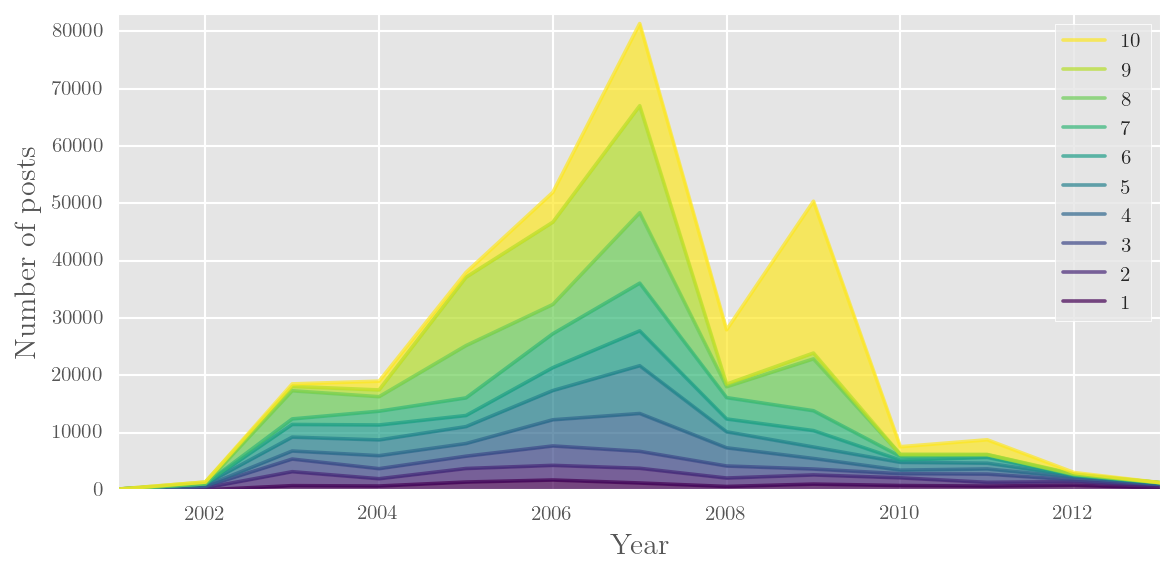
\includegraphics[width=0.75\textwidth]{../images/posts-by-year.png}
\caption[Number of posts in the \emph{Longitudinal Structure}]{Number of posts in the \emph{Longitudinal Structure} by membership stage}
\label{fig:stage_year}
\end{figure}

\begin{figure}[htb]
\centering
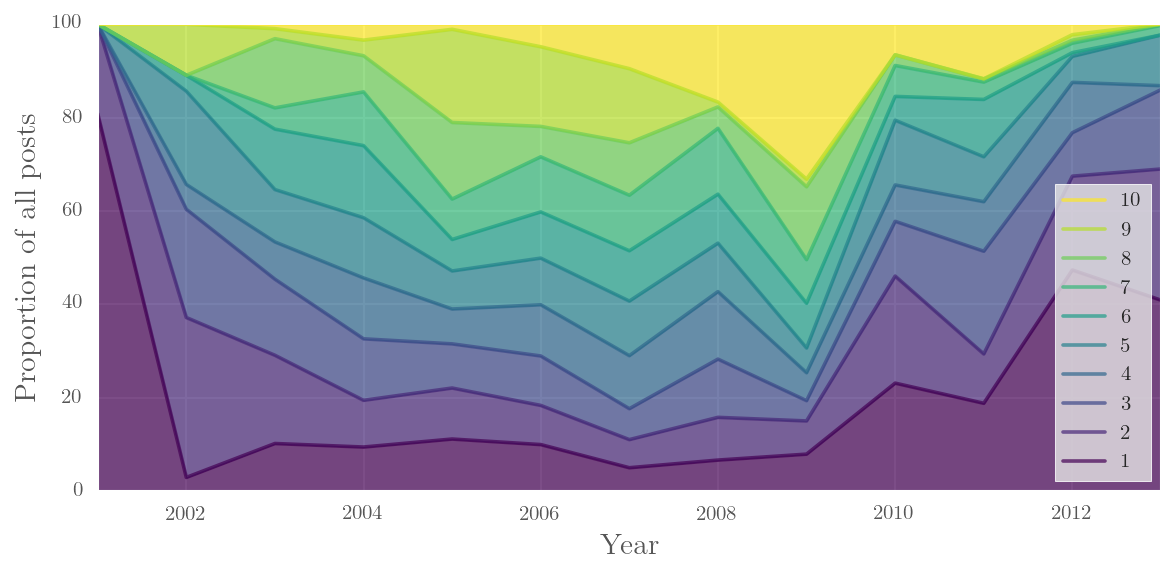
\includegraphics[width=0.75\textwidth]{../images/posts-by-year-filled.png}
\caption[Relative number of posts in the \emph{Longitudinal Structure}]{Relative number of posts in the \emph{Longitudinal Structure} by membership stage}
\label{fig:stage_year_filled}
\end{figure}

\begin{figure}[htb]
\centering
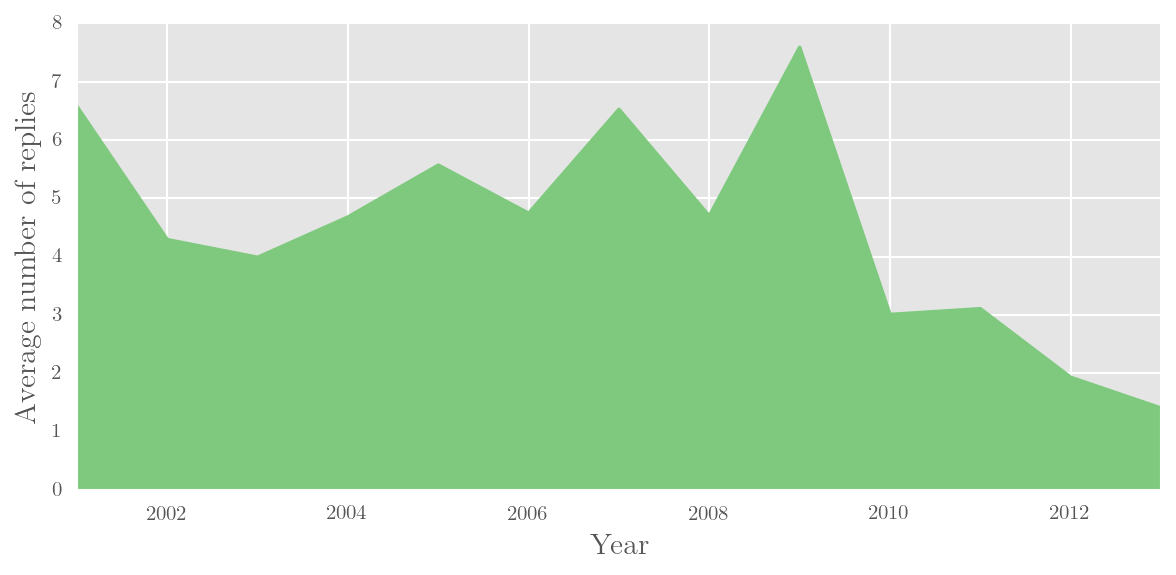
\includegraphics[width=0.75\textwidth]{../images/avg-replies.png}
\caption[Replies to new threads in the \emph{Longitudinal Structure}]{Average number of replies to new threads in the \emph{Longitudinal Structure}}
\label{fig:avg_replies}
\end{figure}

Figure \ref{fig:stage_year} uses the Longitudinal Structure to provide an overview of the amount of activity within the \gls{Forum} by year. The number of \glspl{post} steadily increases until 2009, at which point there is a similarly steady decline. Figure \ref{fig:stage_year_filled} shows the extent to which different membership stages are represented in the \gls{Forum} in a given year. Having information about the composition of membership stages at different points in time makes it possible to speculate as to what a low or high concentration of veteran members does to language use in the \glslink{Forum}{community} as a whole. This is not, however, a focus of the thesis.

Figure \ref{fig:stage_year_filled} shows that in the busiest years of the \gls{Forum}'s history, veteran \glspl{member} made proportionally more \glspl{post}.\endnote{It is important to remember that since a user must \gls{post} 560 or more times to enter the last stage of membership, veteran \glslink{member}{users} in the earlier years of the \gls{Forum}'s existence are bound to be less common.}~These members then gradually stop \glslink{post}{posting}; in the latest years sampled, many newcomers \gls{post} a question, but receive no reply (see Figure \ref{fig:avg_replies}). Combined, the smaller number of overall \glspl{post}, the departure of veteran \glspl{member}, and lack of follow\hyp{}up to new \glspl{thread} are taken as indicators that the \gls{Forum} is moribund.

\subsubsection*{\emph{Comparative Structure}}

The final structure, the \emph{Comparative Structure} consists of two subcorpora. In the first are the first 30 \glspl{post} of \glslink{member}{users} who did not progress beyond 30 \glspl{post} (`Dropouts'). In the second are the first 30 \glspl{post} of those \glslink{member}{users} who did (`Future veterans'). This structure makes it possible to \emph{check for differences in the early\hyp{}stage language of future\hyp{}veterans and early dropouts}. It is designed to address the possibility that there is a pre\hyp{}existing difference in the linguistic features of \glspl{member} who drop out early and \glspl{member} who become veterans.

\begin{table}[htb]
\centering
\footnotesize
\begin{tabular}{lrrrrrrr}

\toprule
{} &  Characters &   Tokens &    Words &  Closed class &  Open class &  Clauses &  Sentences \\
\midrule
Dropout        &    $15,480,624$ &  $4,478,616$ &  $3,883,247$ &  $2,293,005$ &           $2,185,611$ &  $1,011,519$ &     $252,142$ \\
Fut. vet. &    $17,070,684$ &  $4,946,441$ &  $4,257,184$ &  $2,559,998$ &           $2,386,443$ &  $1,120,599$ &     $271,185$ \\
\bottomrule
\end{tabular}
\caption{Shallow features in the \emph{Comparative Structure}}
\label{tab:shallow_C}
\end{table}


\section{\texttt{corpkit}: tools for corpus building and analysis} \label{sect:corpkit}

Data analysis involved the use of a purpose\hyp{}built \texttt{Python}\hyp{}based toolkit, \texttt{corpkit}. In this section, I explain the need for the tool, its development, core functionality, and significance within the research area. Complete documentation of its programmatic, graphical and interpreter interfaces is available via \texttt{\href{https://www.github.com/interrogator/corpkit}{https://www.github.com/interrogator/corpkit}}.

\subsection{Rationale for tool development}

Before analysing the \gls{corpus} data, a survey of existing tools for corpus analysis was conducted, with a number of criteria in mind:

\begin{enumerate}
\item Feature-richness: ability to perform lemmatisation, lexical and grammatical searches, handling of plain text, \gls{POS} tags, constituency and dependency parses
\item Automatability: ability to loop through subcorpora, or through lists of queries, or cycling through options such as lemmatisation, removal of closed\hyp{}class words, etc.
\item Flexibility: ability to add to wordlists, edit interrogation results (merging search results, spanning subcorpora, etc.)
\item Sensitivity to functional grammar(s): ability to operationalise functional linguistic notions when interrogating corpora and editing results (i.e. locate Events within Processes)
\item Visualisation: ability to generate useful visualisations of language use without the need to export data from the tool
\end{enumerate}
%
In addition to these selection criteria, preference was given to resources that were:
%
\begin{enumerate}
\item Open-source, freely available, non\hyp{}proprietary
\item Command\hyp{}line based, rather than graphical (to facilitate automation, replicability, etc.)
\end{enumerate}
%
With these criteria in mind, the following tools were tested for suitability:
%
\begin{multicols}{3}
\begin{enumerate}
\item \texttt{NLTK}
\item \texttt{WMatrix}
\item \texttt{AntConc}
\item \texttt{CasualConc}
\item \texttt{Wordsmith Tools}
\item \texttt{Sketch Engine}
\item \texttt{UAM Corpus Tool}
\item \texttt{Tregex}
\item \texttt{\gls{CWB}\slash CQP}
\end{enumerate}
\end{multicols}
%
\noindent Though individual features from each tool were useful, none satisfied all selection criteria. Shifting between tools during different stages of the investigation was also unfeasible, as much interrogation was exploratory, iterative, or cyclical. \texttt{UAM Corpus Tool}, while able to handle multiple subcorpora, and while providing systemic\hyp{}functional conversions of \texttt{Stanford CoreNLP} parses, was also not suitable, as it:
%
\begin{enumerate}
\item Struggled to cope with the size of the corpus\endnote{\texttt{UAM Corpus Tool}'s creator, Mick O'Donnell, has since re\hyp{}factored the tool to handle very large datasets.}
\item Had stability issues (for example, when exporting interrogation results)
\item Is \gls{GUI}\hyp{}based, and cannot be scripted
\item Does not grant the user direct access to the systemic\hyp{}functional parses or the parser itself, making it difficult to verify the accuracy of converted parses\endnote{O'Donnell is preparing to release much of the non\hyp{}\gls{GUI} code as open\hyp{}source (personal communication, 2015).}
\item Requires exporting data in order to sort or visualise results
\end{enumerate}
%
Command\hyp{}line tools such as the \texttt{Open Corpus Workbench} \cite{evert2011twenty} provided the necessary ability to perform iterative and recursive searches, but lacked the ability to extract complex features from full syntactic parser output, and to easily interface with state\hyp{}of\hyp{}the\hyp{}art tools for manipulating and visualising data. \texttt{Tregex} \cite{levy2006tregex}, a search query language for constituency trees, is able to perform complex queries, but does not handle lemmatisation, keyword calculation or advanced result manipulation. \texttt{NLTK} \cite{bird2009natural}, while containing routines for many linguistic tasks, did not provide an interface to parsing or interrogating \texttt{CoreNLP} dependency parser output,\endnote{More recent releases of \texttt{NLTK} have better integration with \texttt{Stanford CoreNLP}.} and did not provide a holistic interface for more general workflows. Given these considerations, the development of purpose\hyp{}built tools was the best solution, providing increased transparency and reproducibility of this investigation, while also being useful for other researchers interested in functional \gls{CL}.

\subsection{Contents of the toolkit}

\texttt{corpkit} is a \texttt{Python} module designed to create and interrogate parsed and structured \glspl{corpus}, edit interrogation results, and to display\slash visualise edited output. It is available as open\hyp{}source software:

\begin{enumerate}
    \item GitHub: \texttt{\href{https://www.github.com/interrogator/corpkit}{https://www.github.com/interrogator/corpkit}}
    \item PyPI: \texttt{\href{https://pypi.python.org/pypi/corpkit}{https://pypi.python.org/pypi/corpkit}}
    \item Documentation: \texttt{\href{http://corpkit.readthedocs.org/}{http://corpkit.readthedocs.org/}}
    \item Standalone app: \texttt{\href{http://interrogator.github.io/corpkit/}{http://interrogator.github.io/corpkit/}}
\end{enumerate} 
%

The toolkit is \emph{object\hyp{}oriented}. Users instantiate \glspl{corpus} as objects, which have methods for parsing, interrogating and concordancing. Interrogations are also objects, which have methods for editing, the calculation of statistics, saving and visualising. A basic workflow using the Python \gls{API} involves the following steps:

%\todo{Workflow as algorithm}

\begin{enumerate}
    \item Create a project to house corpus\slash \glspl{corpus}, saved data, images, wordlists \\ (\texttt{new\_project()} function)
    \item Instantiate plaintext corpus \\ (\texttt{Corpus} class)
    \item Parse plaintext corpus using \texttt{Stanford CoreNLP} \\ (\texttt{Corpus.parse() method})
    \item Interrogate\slash concordance parsed corpus for \glslink{lexicogrammar}{lexicogrammatical} phenomenon \\ (\texttt{Corpus.interrogate()} method)
    \begin{itemize}
        \item Constituency parses via \texttt{Tregex}\slash \texttt{nltk\_tgrep}
        \item Dependency parses via \texttt{pandas}
    \end{itemize}
    \item Edit results \\ (\texttt{Interrogation.edit()} method)
    \begin{itemize}
        \item Keeping, removing, merging entries or subcorpora
        \item Calculating relative frequencies
        \item Sorting, generating statistics, doing linear regression
        \item Keywording
    \end{itemize}
    \item Tabulate, export or visualise edited results \\ (\texttt{Interrogation.visualise()} method)
    \item Save data to project \\ (\texttt{Interrogation.save()} method)
\end{enumerate}
%
\texttt{Interrogation} objects store a dictionary of the parameters that created them, so that they can easily be reproduced. Saved interrogation results are loaded as \gls{corpus} attributes at the beginning of each session, simplifying the process of managing projects involving multiple \glspl{corpus}.

\subsubsection{Key design parameters}

The tool was designed in response to the needs of the case study, to noted shortcomings of existing tools, and to a small body of literature describing needs in the future generation of \gls{corpus} tools \cite[e.g.][]{anthony_critical_2013,anthony_developing_2006,gries_50-something_2013}. \textcite{anthony_critical_2013} provide a succinct summary of needed tool development:

\begin{quote} \small \singlespacing
[Linguistic research] will rely increasingly on large corpora, advanced functionality, and sophisticated statistical methods. \ldots~\Gls{corpus} tool development should be an open source initiative with tool components being developed in a modular fashion. By dividing tool components in this way, it becomes easier for tool functions and features to be extended, modified, or simplified depending on the need' \parencite*[pp.~155--156]{anthony_critical_2013}.
\end{quote}
%
\texttt{corpkit} responds to each of these parameters: it is built to work with \glspl{corpus} of any size, and to allow multiprocessing to speed up queries over very large datasets; it has the most advanced functionality of any corpus interrogation tool to date, with support for parsing, interrogating parser output, and distinguishing between subcorpora and metadata tags or values; it integrates with \texttt{scipy} \cite{scipy2001} and \texttt{pandas} \cite{mckinney_pandas_2010} in order to allow complex mathematical operations; it is free and open\hyp{}source; it is modular, interfacing with dedicated modules for editing, storing and visualising; graphical and command\hyp{}line interfaces tailored to programming and non\hyp{}programming linguists.

\subsection{Interfaces and functionality of the tool}

\texttt{corpkit} includes three different interfaces. The \gls{API} itself, used for all data analysis in the thesis, is the most powerful, but requires knowledge of Python. The other two interfaces---a graphical application, and a natural language interpreter---call the \gls{API} as a backend. These interfaces were developed with the aim of increasing the potential users of the tool to those without a background in computer programming. At the same time, because users can shift freely between interfaces, it was hoped that the tool could facilitate increasingly programmatic workflows in \gls{CL}. In the sections below, I explain the functionality of the tool, giving examples from the \gls{API}. The graphical and interpreter interfaces are introduced later.

\subsubsection{API}

The most complex interface is the \gls{API}, implemented in Python. Through this interface, users can access the full range of methods for a given object, and take advantage of common programming constructs, such as the writing of loops or conditional statements. It is the interface used for the case study itself. The \gls{API} is also the interface with the most potential use for computationally intensive downstream applications in the area of medical\slash clinical \gls{NLP}: it could easily be scripted to automatically parse, categorise and search new data as it becomes available.

\paragraph{\texttt{Corpus}}

The \texttt{Corpus} class models a directory (and optionally, subdirectories) of data files, which may be plain text files or \texttt{CONLL-U} data. Though the toolkit is oriented toward parsed and structured data, basic functionality for interrogating and concordancing is available for plain text \glspl{corpus} as well. \texttt{Corpus} objects have a \texttt{parse} method, which is essentially a wrapper around \texttt{Stanford CoreNLP}, with keyword arguments for annotators, memory allocation and so on. In the example below, a plaintext \texttt{Corpus} object is created and parsed with \texttt{Stanford CoreNLP} using default parameters.

\begin{minted}[linenos,frame=single,xleftmargin=1cm]{python}
from corpkit import Corpus
unparsed = Corpus('forum')
corpus = unparsed.parse()
\end{minted} 
%
This method returns another \texttt{Corpus} object representing the parsed data, which can then be interrogated and concordanced in complex ways. Each subcorpus and file is represented as \texttt{Subcorpus} and \texttt{File} objects respectively, which can also be interrogated and concordanced:

\begin{minted}[linenos,frame=single,xleftmargin=1cm]{python}
parsed['01']
# <corpkit.corpus.Subcorpus instance: 01>
parsed['01'].files[245]
# <corpkit.corpus.File instance: thread-4450244.txt.conll>
\end{minted}

\paragraph{Speaker segmentation}

One innovation in \texttt{corpkit}'s \texttt{parse} method is the addition of speaker segmentation. The \texttt{parse} method has a \texttt{speaker\_segmentation} argument, which will add speaker names to \texttt{CoreNLP} output, provided they are delineated with a colon at the start of a line, or by \gls{HTML}\slash \gls{XML} tags in the text. The process of speaker segmentation involves:

\begin{enumerate}
\item Creating a duplicate corpus with names removed
\item Parsing the duplicated corpus
\item Using character offset metadata in the parser output to find the original line in the duplicated text
\item Lifting the speaker name from the original corpus
\item Adding the speaker name to the parser output
\end{enumerate}
%
% todo: revise for truth
The Bipolar Forum Corpus also has speaker names included in the annotations, so that interrogations can be restricted to a particular \glslink{member}{user} or set of \glslink{member}{users}. It is therefore also possible to look for differences between how newcomer and veteran \glslink{member}{users} use language in one or more \glspl{thread}. At a broader level, this method makes it possible to computationally model register features of dialogic text, facilitating context\hyp{}responsive parsing (see Chapter \ref{chap:implications}). Such tasks are beyond the scope of the current investigation, however.

\paragraph{\texttt{Corpus.interrogate() method}}

As explained in the previous chapter, \gls{CL} is centrally concerned with extracting frequency information from texts. Generally speaking, researchers are interested in either counting the occurrences of a particular linguistic feature in each subcorpus (e.g. counting a particular word or grammatical feature), or in counting the possible realisations of a linguistic feature (counting the frequencies of every word that is a noun, or every subject in a passive construction). Perhaps surprisingly, few tools provide an interface for doing this kind of searching or counting. \texttt{corpkit} focusses on iterating over subcorpora, extracting complex \glslink{lexicogrammar}{lexicogrammatical} features, and tabulating the results.

The \texttt{Corpus.interrogate()} method, more precisely, centres on a three\hyp{}step process of \emph{searching}, \emph{excluding} and \emph{showing} (Figure \ref{fig:mod-of-doc}). Searching and excluding involve the specification of one or more combinations of \emph{search objects} and regular expression or wordlist\hyp{}based patterns to match. Search objects are broken down into a token of interest (i.e. a token, its governor, one of its collocates, etc.) and its attributes (i.e. its word form, its lemma form, its \gls{POS}, etc.---see Table \ref{tab:search-exclude-show}). The \texttt{GL} search object, for example, searches for any lemma form matching a pattern, returning the ID of its dependent(s). After each search criterion has been processed, indices of tokens are removed if they appear fewer times than the total number of search criteria---that is, tokens must match all search criteria by default. Then, any explicit excluding is performed, using the same syntax as searching: if a token matches the exclusion criteria, it is filtered from the set of matches. After exclusion is complete, a function is called that determines how to represent the search matches. If the user inputs \mintinline{python}{show=[I, P, L, GL]}, the program will output the index, \gls{POS}, lemma form and governor's lemma form of a match (e.g. \mintinline{python}{'2/NNS/user/be'}). Results are returned as a two\hyp{}dimensional array of counts for each shown object in each subcorpus. Figure \ref{fig:mod-of-doc} provide an examples of this method for constituency and dependency parses. In both cases, lemmatised adjectives modifying terms for doctors are returned. This produces the results shown in Table \ref{conc:adj_mod_doc_example}.

\begin{table}[htb]
\centering
\small
\begin{tabular}{lrrrrrrrr}
\toprule
{} & Match & Gov. & Dep. & Coref Head & N-gram & Collocate & 1L & 1R \\
\midrule
Word          &     \texttt{W} &       \texttt{GW} &        \texttt{DW} &        \texttt{HW} &     \texttt{NW} &        \texttt{BW} &        \texttt{-1W} &        \texttt{-1W} \\
Lemma          &     \texttt{L} &       \texttt{GL} &        \texttt{DL} &        \texttt{HL} &     \texttt{NL} &        \texttt{BL} &        \texttt{-1L} &        \texttt{-1L} \\
Function       &     \texttt{F} &       \texttt{GF} &        \texttt{DF} &        \texttt{HF} &     \texttt{NF} &        \texttt{BF} &        \texttt{-1F} &        \texttt{-1F} \\
POS tag         &     \texttt{P} &       \texttt{GP} &        \texttt{DP} &        \texttt{HP} &     \texttt{NP} &        \texttt{BP} &        \texttt{-1P} &        \texttt{-1P} \\
Wordclass      &     \texttt{X} &       \texttt{GX} &        \texttt{DX} &        \texttt{HX} &     \texttt{NX} &        \texttt{BX} &        \texttt{-1X} &        \texttt{-1X} \\
%Distance from \texttt{root}       &     \texttt{R} &       \texttt{GR} &        \texttt{DR} &        \texttt{HR} &     \texttt{NR} &        \texttt{BR} &        \texttt{-1R} &        \texttt{-1R} \\
Index          &     \texttt{I} &       \texttt{GI} &        \texttt{DI} &        \texttt{HI} &     \texttt{NI} &        \texttt{BI} &        \texttt{-1I} &        \texttt{-1I} \\
Sent. index &     \texttt{S} &       \texttt{GS} &        \texttt{DS} &        \texttt{HS} &     \texttt{NS} &        \texttt{BS} &        \texttt{-1S} &        \texttt{-1S} \\
Named entity &     \texttt{E} &       \texttt{GE} &        \texttt{DE} &        \texttt{HE} &     \texttt{NE} &        \texttt{BE} &        \texttt{-1E} &        \texttt{-1E} \\
\bottomrule
\end{tabular}
\caption[Possible object--attribute combinations]{Possible object--attribute combinations to search, exclude or show}
\label{tab:search-exclude-show}
\end{table}


\begin{figure}[htb]
\begin{minted}[linenos,frame=single,xleftmargin=1cm]{python}
# define tree-based (tregex) query
tquery = {T: r'/JJ.?/ > (NP <<# (/NN.?/ < /^(doctor|dr\.|p*doc)s*/))'}
# search the corpus, output matching lemmata
t_doc = corpus.interrogate(tquery, show=L)
# via dependencies: search func, gov. lemma, gov. pos
dquery = { F: 'amod',
          GL: r'^(doctor|dr.|p*doc)s*',
          GP: r'^N'}
# search the corpus, output matching lemmata
d_doc = corpus.interrogate(dquery, show=L, conc=True)
# show table
print(d_doc.results.to_latex(columns=range(4)))
\end{minted}
\caption[Using the \texttt{corpkit} API]{Using \texttt{corpkit} find Epithets\slash Classifiers of health professionals in the Bipolar Forum Corpus}
\label{fig:mod-of-doc}
\end{figure}

\FloatBarrier


\begin{table}[htb]
\centering
\small
\begin{tabular}{lrrrr}

\toprule
Subcorpus &  \emph{new} &  \emph{good} &  \emph{different} &  \emph{regular} \\
\midrule
$01$ &   $58$ &    $16$ &         $29$ &       $12$ \\
$02$ &   $53$ &    $25$ &         $19$ &       $15$ \\
$03$ &   $45$ &    $17$ &         $11$ &       $13$ \\
$04$ &   $60$ &    $21$ &         $16$ &       $19$ \\
$05$ &   $57$ &    $30$ &         $ 8$ &       $12$ \\
$06$ &   $57$ &    $21$ &         $15$ &       $18$ \\
$07$ &   $65$ &    $25$ &         $13$ &       $21$ \\
$08$ &   $90$ &    $29$ &         $ 8$ &       $22$ \\
$09$ &   $51$ &    $14$ &         $15$ &       $11$ \\
$10$ &   $84$ &    $40$ &         $20$ &       $ 6$ \\
\bottomrule
\end{tabular}
\caption{Adjectives modifying doctor words}
\label{conc:adj_mod_doc_example}
\end{table}

\paragraph{Concordancing}

Concordancing is the process of bringing up a vertically aligned set of query matches, with a window of characters or words on either side (see Section \ref{sect:concordancing}). Concordancing has typically been lexically oriented: users search for words via simple or regular expression queries. Some concordancers allow \gls{POS} tagged datasets (e.g. \emph{AntConc}); command\hyp{}line tools may allow searching of information such as lemma forms. \texttt{corpkit}, however, extends concordancing to the same range of features as can be searched and shown via lexicogrammatical querying; in fact, the tool treats concordancing and interrogating as two variants of the same task of interrogation, where concordances are the (monomodal) full text, optionally alongside grammatical information, and \glslink{lexicogrammar}{lexicogrammatical} interrogations are the frequency counts for searches, reduced to their smallest meaningful form. For this reason, both practices are performed by the same method. In the previous code example, the \mintinline{python}{conc=True} keyword argument is responsible for generating the concordance shown in Table \ref{conc:mod_doc_example}.

\FloatBarrier

\begin{table}[htb]
\footnotesize
\begin{tabular}{lrll}

\toprule
     ASHEA & i mention he has not seen this &  actual    &  doctor for at least 2 years .       \\
  ASchwagz &                  i have seen 3 &  different &  family doctors , 2 different psychi \\
  ASchwagz & 3 different family doctors , 2 &  different &  psychiatrists and 1 endocrinologist \\
    Allibo &   of course , when i called my &  primary   &  care dr. to prove the urologist wro \\
   AllieTr &                         find a &  good      &  doctor .                            \\
    Althea & thyroid meds , psychiatrist or &  other     &  doc ???                             \\
 AmySue902 &           through out the last &  few       &  years i have been diagnosed bd by a \\
 AmySue902 &  i have been diagnosed bd by a &  few       &  other doctors but have always refus \\
 AmySue902 & have been diagnosed bd by a few &  other    &  doctors but have always refused the \\
     Angie &                       i have a &  great     &  doctor that only charges me \$ 50 a  \\
\bottomrule
\end{tabular}
\caption{Concordancing adjectives modifying \emph{doctor}}
\label{conc:mod_doc_example}
\end{table}

\paragraph{\texttt{Interrogation.visualise()} method}

Visualisation makes it possible to compress large amounts of complex numerical information into forms that aid in the recognition of patterns. Visualisation of linguistic data has two main purposes. First, it can be used to help the researcher to understand and interpret data. Second, it can be used to present results to readers. Most corpus tools require data to be exported and visualised in dedicated tools. This stifles the ability to use visualisation as a way to generate insights, prioritising only the use of visualisation to display data for readers. \texttt{corpkit}, on the other hand, contains an interface tailored specifically to the visualisation of linguistic data, via \texttt{matplotlib} \cite{matplotlib_2007}. Users can thus produce visualisations without leaving \texttt{corpkit}, making it possible to generate visualisations for both purposes.

The method allows bar charts, pie charts, line charts, area charts, and so on. Data can be stacked or shown cumulatively. The interface simplifies titling, axis labelling, legend placement, figure sizing, as well as the use of dozens of colours and styles. As used in Chapter \ref{chap:experiential}, heatmaps can also be created. These can be constant or diverging, and work with any kind of frequency (absolute, relative, keyness, etc.) that can be calculated with the tool.

%\paragraph{\texttt{Interrogation.multiplot()} method}

%The visualisation capabilities of the module can be extended through the \texttt{multiplot} method, which allows dual display of entire Interrogations alongside individual data points. This makes it possible to visualise the general behaviour of a feature alongside its realisations---in systemic terms, to show two points along the cline of instantiation at the same time.

%The method allows the user to pass in two dictionaries: one for the larger plot (the feature), and another for the smaller plots (the realisations). Additional arguments can dictate the layout of the figure. Separate data can also be passed in for each, so that two kinds of statistic can be presented (i.e. relative frequency vs. keyness). %As an example, Figure n shows ...

\paragraph{Automating workflows}

The tools were developed to facilitate automatic processing of the dataset, with as little need for human intervention and manual analysis as possible. This means that the tool must automate the kinds of things that corpus linguists typically perform by hand. To give an example, a researcher may determine that \emph{wonder} is a frequent or apparently interesting process in a \gls{corpus}. In response, he\slash she may:

%For discourse analysts,\endnote{Lexicographers and language learners also use concordances, but with different motivations that are not relevant here.} 

\begin{enumerate}[noitemsep,topsep=0pt]
\item Count frequency and calculate keyness of \emph{wonder}
\item Concordance \emph{wonder}
\item Curate results:
\begin{itemize}[noitemsep,topsep=0pt]
\item Remove instances where \emph{wonder} is nominal
\item Remove instances where \emph{wonder} is not a process
\end{itemize}
\item Identify a phenomenon of interest in clauses with \emph{wonder} as process, e.g.
\begin{itemize}[noitemsep,topsep=0pt]
\item Subjects of \emph{wonder}
\item Modification of \emph{wonder} through modals, adverbs and negation
\end{itemize}
\item Exclude non\hyp{}relevant examples
\item Read through concordance lines, count results, describe patterns, contrast with other features \ldots
\end{enumerate}
%
In this kind of workflow, concordancer output is used both to get a sense of how a \glslink{lexicogrammar}{lexicogrammatical} feature behaves, and to do content analysis or thematic categorisation. There are limits, however, to the number of examples human coders can process. Using parsed \glspl{corpus}, however, it is possible to automate a much larger portion of the method. In \texttt{corpkit}, the user can search for any participant or modifier that has a governing lemma \emph{wonder} that fills the role of \emph{process}. The \texttt{edit} method can then be used to create relative frequencies, and the \texttt{visualise} method to plot the top results. Concordancing, in this kind of workflow, can be done to ensure that the query is matching the expected kinds of patterns in text, or to provide a selection of contextualised examples for the reader. Finally, it is important to note the potential power of iteration that comes with the programmatic approach: the developed code (Figure \ref{fig:wonder-code}) could be placed inside a loop, so that processes other than \emph{wonder} can be investigated with little additional effort (e.g. \mintinline{python}{for verb in ['wonder', 'appreciate', 'care', 'need']} \texttt{\dots}).

\begin{figure}[H]
\begin{minted}[linenos,frame=single,xleftmargin=1cm]{python}
from corpkit.dictionaries import processes, roles
# a list of verbal processes
verbal = processes.verbal.lemmata
# match nsubj of these processes as root
criteria = {GL: 'wonder',    # governor lemma
            GF: roles.event, # governor function
            GP: r'^V.*',     # governor pos
             F: roles.modifier + roles.participant1} # function
# show function and lemma form
data = corpus.interrogate(search=criteria, show=[F, L])
# make relative frequencies
rel_data = data.edit('%', SELF)
# create 2*2 lineplot with subplots
rel_data.visualise(subplots=True,layout=(2,2))
# make table
print(rel_data.results[:4,:4].to_latex())
\end{minted}
\FloatBarrier
\caption[Example investigation code]{Example investigation code: searching dependency parses for participants and circumstances in \emph{wonder} as process}
\label{fig:wonder-code}
\end{figure}

\begin{figure}[H]
\centering
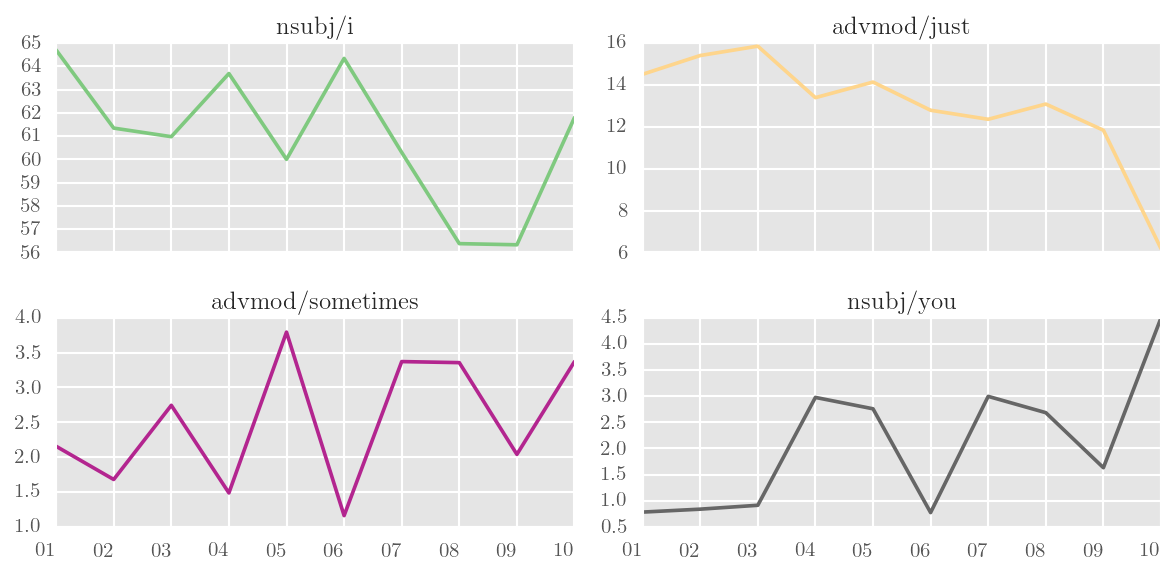
\includegraphics[width=0.70\textwidth]{../images/wonder-example.png}
\caption[Example figure]{Example figure: participants and circumstances for \emph{wonder} as process}
\label{fig:wonder_example_fig}
\end{figure}

\begin{table}[H]
\footnotesize
\begin{tabular}{lrrrr}

\toprule
{} &    nsubj &  advmod &  advmod &  nsubj \\
{} &    i &  just &  sometimes &  you \\
\midrule
01 &  64.705 &  14.509 &  2.156 &  0.784  \\
02 &  61.344 &  15.406 &  1.680 &  0.840  \\
03 &  60.975 &  15.853 &  2.743 &  0.914  \\
04 &  63.690 &  13.392 &  1.488 &  2.976  \\
05 &  60.000 &  14.137 &  3.793 &  2.758  \\
\bottomrule
\end{tabular}
\caption[Example result]{Example result as a multi\hyp{}indexed two dimensional array}
\end{table}

%\begin{minted}[linenos,frame=single,xleftmargin=1cm]{python}
%conc = corpus.concordance(search={GL: doc, F: funcs}, show=[F, L])
%conc.format(n=10, columns=[L, M, R], kind=L)
%\end{minted}

\begin{table}[H]
\footnotesize 
\ttfamily
\begin{tabular}{lrll}

\toprule
0 &                                    &  nsubj\slash i          &  aux\slash be root\slash wonder .\slash , dobj\slash what de \\
1 &                                    &  nsubj\slash i          &  root\slash wonder det\slash the amod\slash same dobj\slash  \\
2 &                                    &  nsubj\slash i          &  aux\slash be advmod\slash just root\slash wonder det\slash  \\
3 &                      nsubj\slash I aux\slash be &  advmod\slash just      &  root\slash wonder det\slash what nsubj\slash person a \\
4 &                                    &  nsubj\slash i          &  root\slash see poss\slash my dobj\slash doc .\slash on prep \\
5 &   nsubj\slash he root\slash say &  nsubj\slash he         &  aux\slash be ccomp\slash wonder mark\slash if nsubj\slash h \\
6 &                                    &  nsubj\slash i          &  aux\slash be root\slash wonder mark\slash if nsubj\slash st \\
7 &                                    &  nsubj\slash i          &  advmod\slash sometimes root\slash wonder mark\slash i \\
8 &                            nsubj\slash I &  advmod\slash sometimes &  root\slash wonder mark\slash if nsubj\slash i aux\slash hav \\
9 &                                    &  nsubj\slash i          &  root\slash wonder mark\slash if nsubj\slash anyone ad \\
\bottomrule
\end{tabular}
\caption[Example concordance]{Example concordance: participants and circumstances in \emph{wonder} process}
\label{conc:wonder_example}
\end{table}

\paragraph{Keywording}

Keywording is a common means of determining which words in a \gls{corpus} are unusually frequent, based on a particular statistical measure such as log\hyp{}likelihood, mutual information or percentage difference (see Section \ref{sect:keywording}). Traditional tools treat keywording as a kind of \gls{corpus} search or interrogation. Keywording is better understood, however, as a statistical operation performed on absolute frequency interrogation results. The new method facilitates using any of these statistical measures in two novel ways. First, keywording is opened up to the full power of the \texttt{search, exclude and show} pipeline. This allows keywording of grammatical participants, or of \gls{POS}\hyp{}lemma pairs. Keywords for n\hyp{}grams, groups and phrases can also be calculated. It becomes possible, therefore, to target particular kinds of constructions, and avoid the use of arbitrary stopword lists. Second, keywords can be calculated in subcorpora using the entire \gls{corpus} as the reference material. This makes it possible to avoid using reference \glspl{corpus}, which are theoretically problematic (See Section \ref{sect:cl-shortcomings}).

\paragraph{Wordlists}

%  (see \texttt{\href{https://github.com/interrogator/corpkit/tree/master/dictionaries}{https://github.com/interrogator/corpkit/tree/master/dictionaries}})
\texttt{corpkit} is designed to be used in tandem with a series of included wordlists. These wordlists were adapted from numerous resources, including the \emph{Process Type Database} \cite{neale_more_2002} and \texttt{pattern.en} \cite{pattern_2012}. This makes it possible to match or remove words of certain types from further analysis. Wordlists include:
%
\begin{enumerate}
\item Closed class words:
\begin{itemize}
\item Pronouns
\item Prepositions
\item Articles
\item Determiners
\item Connectors, conjunctions
\item Modals
\end{itemize}
\item Systemic\hyp{}functional Process Types:\endnote{Original list provided by Mick O'Donnell. Extending these lists to other Process Types is a key future aim.}~
\begin{itemize}
\item Mental
\item Verbal
\item Relational
\item Material
\end{itemize}
\item Conversion\slash normalisation
\begin{itemize}
\item UK\slash US spelling conversion
\item Manual lemmatisation (to augment\slash correct automatic lemmatisation errors)
\end{itemize}
\item Grammar conversion (where possible): from Universal Dependency labels \cite[see][]{nivre_towards_2015} systemic\hyp{}functional labels
\end{enumerate}
%
Each wordlist is a \texttt{Wordlist} object, which has methods for generating verb inflections (via \texttt{WordNet}) or generating regular expressions to match list items:

\begin{minted}[linenos,frame=single,xleftmargin=1cm]{python}
from corpkit.dictionaries.process_types import processes
print(processes.verbal.lemmata[:5])
# ['accede', 'add', 'address', 'admit', 'advise']
print(processes.verbal.words[:5])
# ['accede', 'acceded', 'accedes', 'acceding', 'add']
print(processes.verbal.lemmata[:5].as_regex(boundaries='line'))
# '(?i)^(accede|add|address|admit|advise)$'
\end{minted}
%
Every list can be used as criteria for interrogating \glspl{corpus} or editing results. In the graphical and interpreter interfaces, new wordlists can be interactively created, inflected and saved for later use.

%\subsubsection{Functions}

%\texttt{corpkit}'s core classes and methods are complemented by a number of other functions for saving and loading data, and building regular expressions from wordlists. These are documented online, and in Appendix \ref{appendix:corpkit}.

\paragraph{Additional features}

\texttt{corpkit}'s core classes and methods are complemented by a number of other functions for saving and loading data, and building regular expressions from wordlists. These are documented online, and in Appendix \ref{appendix:corpkit}.

The tool also has broader uses beyond those showcased in this thesis. Language models can be generated from \glspl{corpus}, allowing classification of arbitrary texts by their similarity to texts found in a subcorpus. Such methods make it possible to automatically categorise and interrogate new data. The methods could therefore be applied in near real\hyp{}time to popular online communities, rather than to a community that has completed its lifecycle.

\paragraph{Module dependencies}

\texttt{corpkit} relies heavily on a number of other modules, the most important of which are outlined in Table \ref{tab:corpkit:deps}. Notably, \texttt{Stanford CoreNLP} is used to parse texts, and either \texttt{Tregex} or \texttt{nltk\_tgrep} can be used to query parse trees.\endnote{In this thesis, all constituency queries use \texttt{Tregex}, which has a richer syntax, and is faster.} \texttt{pandas} is another key dependency, being used to store both parser output and search results.

%\texttt{https://github.com/wroberts/nltk_tgrep}

\begin{table}[htb]
\centering
\small
\begin{tabular}{ll}

\toprule
Task                         & Tool  \\ 
\midrule
Tokenisation                 & \texttt{CoreNLP, NLTK} \\     
Lemmatisation (dependencies) & \texttt{Stanford CoreNLP}, \texttt{WordNet} \\
%Lemmatisation (constituencies) & \texttt{NLTK}\slash \texttt{WordNet} \\ 
\gls{XML} manipulation             & \texttt{CoreNLP\_XML}  \\ 
Parse tree traversal         & \texttt{Tregex}, \texttt{nltk\_tgrep}  \\ 
Synonyms, hypernyms, hyponyms & \texttt{NLTK}, \texttt{WordNet}  \\ 
Verb inflections             & \texttt{pattern.en}  \\ 
Linear regression   & \texttt{scipy}          \\ 
Visualisation                & \texttt{matplotlib}, \texttt{pandas}, \texttt{mpld3}  \\ 
Result manipulation          & \texttt{pandas}    \\ 
Multiprocessing              & \texttt{joblib}  \\ 
\bottomrule
\end{tabular}
\caption{Tasks performed in \texttt{corpkit}}

\label{tab:corpkit:deps}
\end{table} 

\subsection{Alternative interfaces}

Though the \gls{API} was used for the analysis of the \glslink{Forum}{Bipolar Forum} \Gls{corpus}, two other inferfaces were also created, in order to maximise the utility of the tool for researchers without expertise in computer programming, or, more specifically, in Python. The first is a graphical application. The second is a natural language interpreter, which parses commands entered by the user and invokes the \gls{API}. These are described in the following two sections.

\subsubsection{Graphical interface}

The simplest of the three developed interfaces is the graphical interface, built using \texttt{Tkinter}. It is reminiscent of other standalone graphical tools such as \texttt{AntConc} and \texttt{UAM Corpus Tool}, providing interfaces for file viewing, corpus searching and concordancing. It extends upon \texttt{AntConc} by adding the ability to parse and search parsed texts, and by allowing the user to work with structured or metadata\hyp{}rich collections of text. It extends on \texttt{UAM Corpus Tool} by providing a greater variety of query languages, as well as result editing and visualisation, and more comprehensive project management, with previous processes stored in memory, so that they may be viewed, saved or discarded. Figure \ref{fig:gui-screenshots} shows the main tabs. Not shown are the \emph{Build} tab (which also visualises parsed sentences), and numerous pop\hyp{}up windows for wordlist creation, thematic category building, and project management.

\begin{figure}[htb]

  \begin{minipage}[b]{0.5\linewidth}
    \centering
    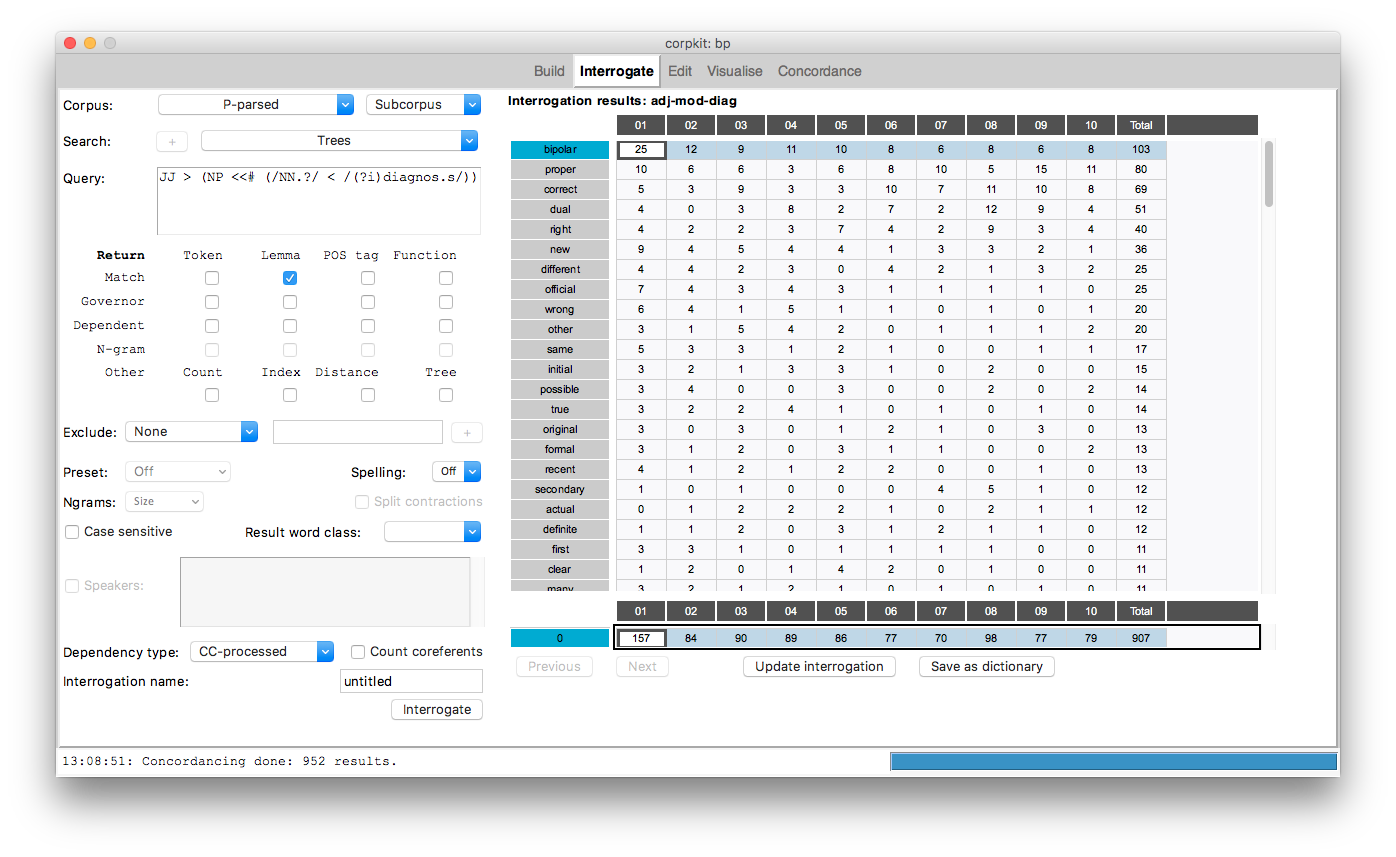
\includegraphics[width=.98\linewidth]{../images/interro} 
    %\caption{Interrogating} 
    \vspace{1ex}
  \end{minipage}%%
  \begin{minipage}[b]{0.5\linewidth}
    \centering
    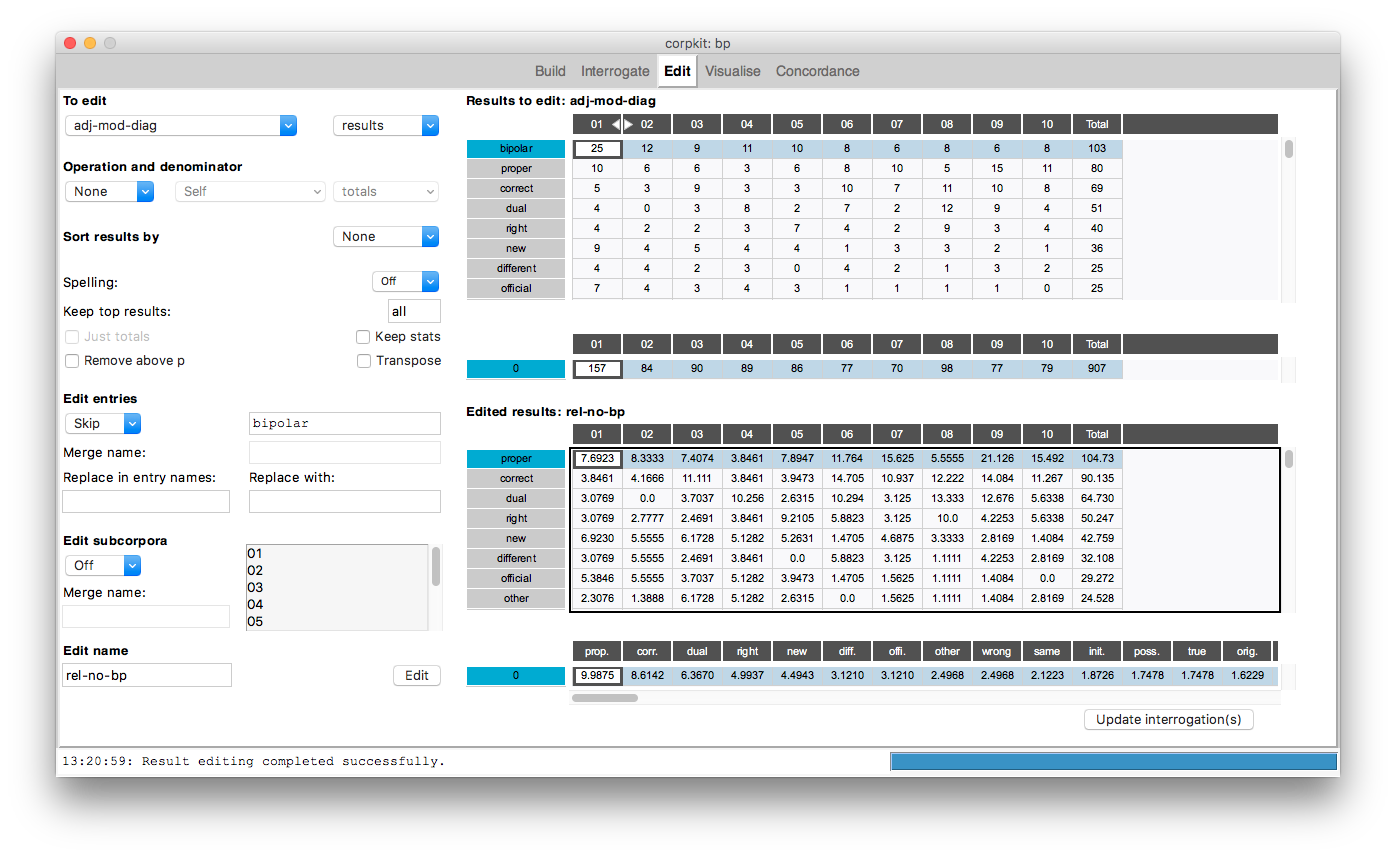
\includegraphics[width=.98\linewidth]{../images/edit} 
    %\caption{Editing} 
    \vspace{1ex}
  \end{minipage} 
  \begin{minipage}[b]{0.5\linewidth}
    \centering
    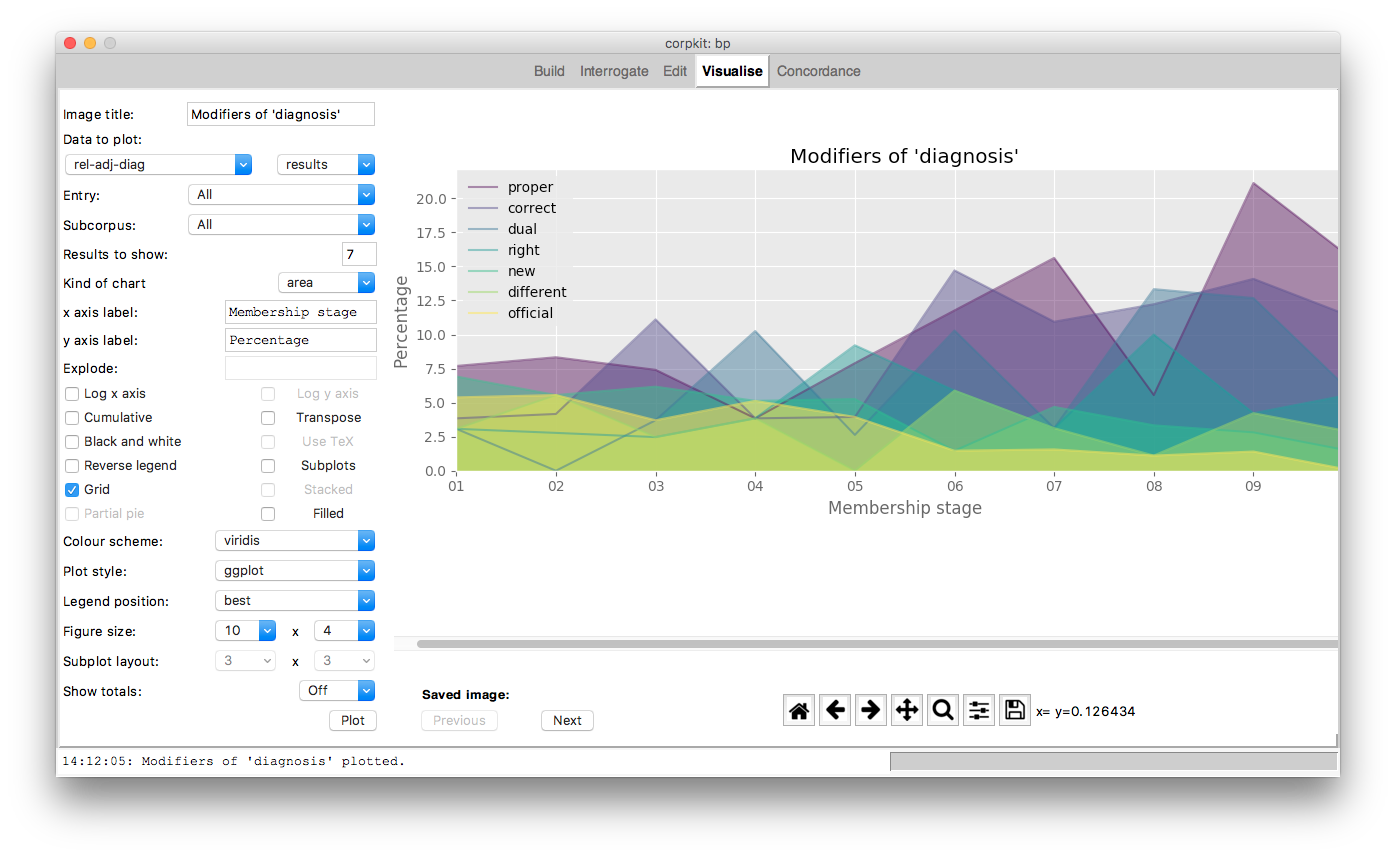
\includegraphics[width=.98\linewidth]{../images/plot} 
    %\caption{Visualising} 
    \vspace{1ex}
  \end{minipage}%% 
  \begin{minipage}[b]{0.5\linewidth}
    \centering
    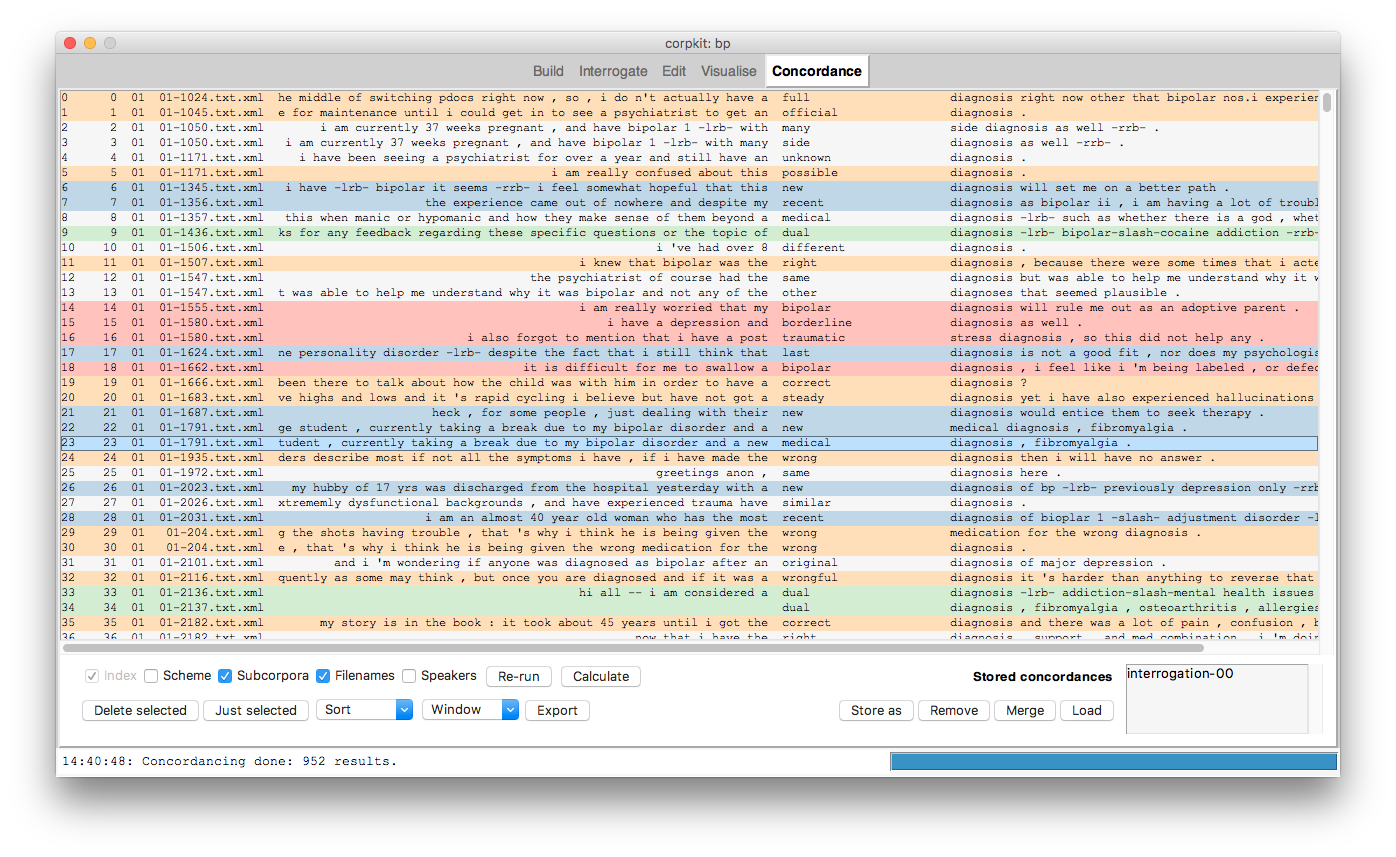
\includegraphics[width=.98\linewidth]{../images/conco} 
    
    \vspace{1ex}
  \end{minipage} 
  \caption{Screenshots from \texttt{corpkit}'s graphical interface}
  \label{fig:gui-screenshots} 
\end{figure}

\subsubsection{Interpreter}

The other alternative interface is a natural language interpreter, which allows the user to type in imperative commands for \texttt{corpkit} to perform. It is reminiscent of the \gls{CWB}. Like the \gls{CWB}, it allows the user to search \glspl{corpus} and annotations in complex ways. The user can create macros and variables, export output, and write scripts that call the tool's functions and methods. It extends upon the functionality of the \gls{CWB} by allowing the user to search fully parsed, rather than \gls{POS}\slash lemmatised text.

\begin{minted}[linenos,frame=single,xleftmargin=1cm,breaklines=true]{bash}
> set bipolar as corpus
> search corpus for governor-lemma matching processes:verbal \
... excluding lemma matching "[write, email, pen]" \
... showing lemma and pos
\end{minted}
%
\noindent The interpreter occupies a middle ground in complexity between the graphical interface and the Python \gls{API}. This makes it particularly suitable as an introduction for corpus linguists to the command line, and programmatic approaches to corpus analysis. Further examples of its syntax can be found throughout Chapter \ref{chap:implications}.

\subsection{Open source development}

A key limitation in previously available \gls{CL} tools addressed by \texttt{corpkit} is in the manner in the tool is provided to the community. In terms of existing \gls{CL} tool, it is notable that most do not provide the end\hyp{}user with access to the source code. At the same time, many are maintained by a single developer. This creates a number of potential problems. First, the software can potentially become a \emph{black box}, where researchers feed in data and interpret output, without understanding what has been done to their data, or how the output was extracted from the input. This can be more or less benign, as when a developer has simply not documented the workings of a feature. At worst, however, the tool may mask its own shortcomings, or remove results that may be important, but apparently uninteresting, or contrary to intuition. At the same time, in closed\hyp{}source software deployment, software users can report, but not fix bugs themselves. This slows down the process of improving a tool, especially in cases where the software is single\hyp{}authored. The second issue that arises in single\hyp{}author, closed\hyp{}source software development is what has been referred to as the \emph{bus factor}, which measures \emph{how many people would need to be hit by a bus in order to make a project unable to proceed?} \cite{cosentino2015assessing}. For many users, switching tools takes significant effort, and involves a learning curve. Making this investment for a tool with an uncertain future may be undesirable. \texttt{corpkit} addresses these problems by being completely open\hyp{}source. Users can not only report bugs, but also fix them. Users may also extend the tool to meet their needs, and request that a developed extension be merged into the master version of the tool. The tool can therefore respond to community needs in a more organic way.

\subsection{Contributions of the toolkit}

The toolkit is a contribution to the \gls{CL} and \gls{SFL} communities, as well as the digital humanities more broadly. It expands on the functionality of many currently available tools, allowing more sophisticated kinds of querying and manipulation than other tools to date. As an example, by allowing the user to forgo reference \glspl{corpus} and stopword lists, its approach to keywording resolves tensions between theoretical orientation of critical\slash functional linguistics (which tend to problematise the notion of balanced\slash representative texts) and keywording (which typically relies on frequency data drawn from reference \glspl{corpus}). \texttt{corpkit} also brings tasks that have typically fallen under the domain of computational linguistics (e.g. lemmatisation, normalisation, parsing, linear regression modelling) to researchers interested in discourse. Despite the notable opposition to lemmatisation and parsing \textcite[by e.g.][]{sinclair_trust_2004}, such perspectives are now uncommon, with increasing recognition that computational methods can enhance the nuance with which the \gls{lexicogrammar} of texts can be probed, and thus the certainty with which claims about \glspl{discourse-semantic} of texts in \glspl{corpus} can be made. Looking at the tool from a computational linguistic perspective, it serves to bring state\hyp{}of\hyp{}the\hyp{}art developments to a new user base, including corpus linguists and discourse analysts. This addresses a problem articulated by \citeauthor{de2008stanford}:

\begin{quote} \singlespacing \small
A major problem for the natural language processing (\gls{NLP}) community is how to make the very impressive and practical technology which has been developed over the last two decades approachable to and usable by everyone who has text understanding need. \dots~ That is, usable not only by computational linguists, but also by the computer science community more generally and by all sorts of information professionals including biologists, medical researchers, political scientists, law firms, business and market analysts, etc. \dots [T]he availability of high quality, easy\hyp{}to\hyp{}use (and preferably free) tools is essential for driving broader use of \gls{NLP} tools \parencite*[p.~1]{de2008stanford}.
\end{quote}

Finally, \texttt{corpkit} is aligned with the emerging areas of digital and programmatic humanities research. It increases transparency and reproducibility of methods and findings: \texttt{Jupyter Notebooks} can be kept under version control and easily shared with others; the graphical interface stores interrogations and edited results in memory during each session, and allows for saving and loading of generated data between sessions. In being free, open\hyp{}source and publicly available, it can be adapted by other researchers, simplifying the process of extending previous research and generating new theory.

\section{Approach to data analysis}

The process of data analysis follows on from the affordances of the developed tools, and from the output of the parsing pipeline: each subcorpus is interrogated via both constituency and dependency parses; results are edited, sorted or merged where necessary to translate findings into meaningful systemic\hyp{}functional terms (insofar as is possible). These findings are then visualised or presented as tables; key points of interest then become the focus of further interrogations. Concordancing and plain-text examples is used where necessary to better understand a given \glslink{lexicogrammar}{lexicogrammatical} phenomenon in co\hyp{}text. As the key area of interest is longitudinal change, linear regression is performed on many interrogation results to calculate trends. This is followed by sorting of the entries by slope, in order to unearth parts of the lexicogrammar that become more or less frequent over time, are turbulent, or remain static.

The approach to analysis can be characterised as \emph{systematic}, \emph{exploratory} and \emph{recursive}:

\subsubsection*{Systematic progression through data}

Interrogation progresses along the cline of instantiation, from broad\slash shallow features to more specific \glslink{lexicogrammar}{lexicogrammatical} realisations. Where possible, investigation of \sctext{Mood} and \sctext{Transitivity} features are also interrogated separately. This `from\hyp{}above' approach is unusual in automatic analysis of text \cite{matthiessen_key_2010}; it is made possible by the combination of full parsing, which gives access to broad features, and the use of theory, which allows targeting expected linguistic sites of change.

\subsubsection*{Exploratory components}

Given the fact that \texttt{corpkit} allows rapid interrogation of the dataset, testing hypotheses is often trivial. As such, features of the \gls{lexicogrammar} that are not expected to be particularly salient (change in determiner use over time, for example) can be tabulated nonetheless. Much of the work of the analysis consists of iteratively exploring the \gls{corpus}, guided by the findings of previous investigations: If past tense appears to be a key feature undergoing longitudinal change, a follow\hyp{}up investigation may count Predicators in past tensed clauses, or look for keywords in these clauses' Adjuncts.

\subsubsection*{Recursivity}

Programmatic methods simplify and expedite the process of querying large datasets. As such, a great deal of recursivity is possible. For example, code can be written that locates key heads of Participants in the \gls{corpus}, searches for processes in which these words are Participants, and so forth. This kind of interrogation was occasionally performed, and is for the most part documented in the accompanying Notebook, rather than in the findings section, as description of methodological steps is unwieldy, compared to simply reviewing\slash rerunning the code.

\subsection{\texttt{IPython} \& the \texttt{Jupyter Notebook}}

\texttt{IPython} is an extension of the Python programming language, designed to allow quick access to Shell commands, to store code output to file and to easily access the output of previous commands \cite{perez2007ipython}. \texttt{Jupyter Notebooks} are web browser based displays of \texttt{IPython} code, as well as code output, headings, text, and multimedia. \texttt{Jupyter Notebooks} are increasingly popular within scientific communities, as they allow code to be contextualised and explained multimodally, and can be easily run by other researchers, ensuring reproducibility of results. Much of the corpus investigation took place via \texttt{IPython} and \texttt{Jupyter Notebooks}. Many key findings from the investigation in this thesis are therefore available in Notebooks available at: \texttt{\href{https://github.com/interrogator/thesis}{https://github.com/interrogator/thesis}}. This Notebook presents methodological processes and code in more depth, and can be used to manipulate the \gls{corpus}, and edit findings and results.

\subsection{Limitations}

The methodology has some limitations. First, it is bound by the speed and accuracy of its dependencies, with shortcomings of other tools inherited into every investigation. Second, it is strongly oriented toward quantitative insights into \gls{corpus} texts, at times homogenising data prior to analysis. This means that bottom\hyp{}up, grounded\hyp{}theory\hyp{}based interpretation of the dataset is not always possible. As such, the emergence of theory from data is perhaps less likely. The methodology also relies on ad\hyp{}hoc translation between three grammars of English---constituency, dependency and the \gls{SFG}. This means that linguistic notions may be simplified, and categories conflated when distinctions are not shared by all grammars. A further consequence is that it is not possible to engage deeply with concepts in \gls{SFL}\slash \gls{SFG} that make it a particularly attractive framework for locating \gls{discourse-semantic} phenomena at risk in a structured \gls{corpus}.

Second, the methodology is also based on relatively simplistic statistical methods. Though the output of interrogations is amenable to complex statistical analysis, here, most results are generated via simple relative frequency or keyness calculation, ordered using least\hyp{}squares regression. This precludes, for instance, predictive applications of the methods, which could reveal which members are likely to progress to veteran stages, or to drop out.

Finally, the methodology is limited to querying the annotated data, and manipulating results. Though strategies for querying the data are more complex than is typical of \gls{CL}\slash \gls{CADS} research, the methodology does not harness a number of emerging methods in computational linguistics for categorising and understanding the content and context of digitised texts. Machine learning approaches to text analysis, for example, allow unsupervised classification of documents based on automatically determined features that theoretically motivated human researchers may not consider. The need for later research to apply state\hyp{}of\hyp{}the\hyp{}art computational techniques is described in Chapter \ref{chap:implications}.

%The complementarity of methods from computational linguistics and discourse analysis is discussed in more detail in Chapter \ref{chap:futuredirections}.

%Topic modelling\endnote{Exploratory topic modelling of the \gls{Forum} contents was performed, using \sctext{Mallet}; spatial considerations prevented the analysis from being presented in this thesis, however.} can be used to automatically group corpus texts by semantic field, based on co-occurrence of lexical items. 

\section{Situating the thesis methodology}

The methods outlined here incorporate components from a number of convergent fields of study, such as text mining, \glslink{CL}{corpus linguistics}, computational linguistics, and the digital humanities. There is no clear line delineating where one of these fields ends and another begins. There is, however, a tendency for digital humanities and \gls{CL} to focus on interpreting specific datasets, while text mining and computational linguistics are primarily interested in the development of tools. A mixed emphasis on methodological innovation and data analysis means that the case study straddles a broad interdisciplinary space. For discourse analysts and corpus linguists, the methods present new ways to engage with well\hyp{}established computational linguistic practices and tools, allowing automatation of work that has previously been possible only through manual analysis. At the same time, text mining and computational linguistics are often concerned with extracting entities and entity relationships, with little consideration of grammatical metaphor, or theories of language and grammar more generally. The developed method thus aims to combine the speed and automation of text mining approaches with the grammatical sensitivity seen in qualitative research. This opens up future research agendas that integrate discourse analysis and state\hyp{}of\hyp{}the\hyp{}art computational linguistic methods.

\section{Chapter summary}

In this chapter, I have outlined and justified the elements of the data collection, approach to analysis and tool development. The following chapters operationalise the methodology in order to investigate language features in the \glslink{forum}{Bipolar Forum}. The analyses is followed by a discussion of findings in Chapter \ref{chap:discuss-bp}.


% why socialisation

%Socialisation is preferred here because it aligns with the systemic\hyp{}functional notion of interaction as interpersonal exchange, with \sctext{Mood} system choices realising an ongoing negotiation of speaker roles. Like \gls{SFL}, socialisation research tends to eschew the cognitive and psychological 

%Because the case study of this thesis does not involve interviews with participants, or any demographic information beyond what is available to all \glspl{member} of the \gls{Forum}, 

%As discussed in Chapter \ref{chap:discussion}, understanding the underlying cause of change is not a prerequisite to modelling or predicting it.
